
\section{Object identification}
The pipeline is usually invoked by running a single command on a night's worth of data. For example, to build the light-curves for the night of, say, \emph{2014-08-21}, then a single command, \texttt{daybuilder.py 2014-08-21} is issued from the command line. The pipeline then runs through all of the data for that night and generates a set of web pages. Depending on the amount of data for that night, this can take 1 hour to 8 hours. 

For each night, an index page, which shows a list of all of the runs in the night along with thumbnail images of the field of view, is created. This allows the user to quickly navigate to the runs that are of interest. In other words, runs that contain science data, rather than acquisitions, biases or flat-fields. By clicking on the thumbnail of the run, the user is taken to a run page. This page shows the full image for each of the three channels. These images are created by stacking all of the individual frames in the run. The page also shows all of the objects that have been identified and have light-curves available. The user can view the light-curves by using the mouse to click on each object, or can scroll through all of the light-curves systematically, by using the left and right arrow keys. 

Scrolling through the light curves in a systematic fashion makes it easy for the user to quickly identify which objects are showing an obvious variability. All of the objects listed below were discovered in this way. 

With this manual inspection it is possible to inspect the light curves at a rate of about 1-2 objects per second. In future, we plan to apply some automated tests to these data to perform the light curve inspection as an integral stage of the automated pipeline. Algorithms to perform these sorts of tests are already known and becoming increasingly more widespread as more large scale sky surveys are being used throughout astronomy research. We plan to re-use work from one or more of these surveys. The recently published Astrokit software, \citep{Astrokit2014} is one tool that we plan to trial in the next version of the automated pipeline. 

\section{Discovered objects}
As discussed in the introduction, chapter \ref{chap:introduction}, we expect to find some new variables in the ULTRACAM archive. These will be objects displaying some kind of variability that is clearly visible over the length of the run and with the cadence of the observations. This will include eclipsing binaries, contact binaries, flare stars, RR Lyrae and $\delta$ Scuti stars. We might also expect to see other short period variables like cataclysmic variables and DV white dwarfs. Since the pipeline is able to track slow moving objects, we can also expect that we will capture some photometry of asteroids that drift through the field.   

We have only inspected approximately 20\% of the reduced data but we have found a few dozen variable objects so far. Below we list a selection of these objects. 

\begin{table}
  \caption{Table of a few of the interesting objects that have been revealed using the automated pipeline. This list contains just a few highlights of the dozen objects detected so far.}
  \begin{tabularx}{15.4cm}{ l  l  l }
  \hline
  Type& ID & Position, J(2000) \\
  \hline
    {W UMa} & 2005-05-10-run012-73 & 11:26:26.2 $-68$:40:50 \\
    {W UMa} & 2013-07-21-run010-48 & 19:44:09.3 $+40$:16:34.0\\
    {W UMa} & 2013-07-21-run010-163 & 19:44:10.1 $+40$:18:09.1\\
    Eclipsing binary & 2013-07-21-run011-162 & 19:54:01.7 $+40$:37:34\\
    $\delta$ Scuti & 2013-07-21-run010-23 & 19:44:19.7 $+40$:16:45.3\\
  \hline
    \parbox[c]{5cm}{Asteroid\\1998 SU139\\ } & \parbox[c]{5cm}{2011-08-26-run014-110\\  } & \parbox[c]{5cm}{20:51:12.0 $-08$:31:25\\ at MJD=55800.038}\\
    \parbox[c]{5cm}{Asteroid\\9108 Toruyusa (1997 AZ6) } & \parbox[c]{5cm}{2009-01-04-run024-61\\}& \parbox[c]{5cm}{08:04:52.3 $+16$:18:10.6\\at  MJD=54836.26642}\\

  \hline
  \end{tabularx}
  \label{tab:newobjects}
\end{table}


\begin{table}
  \centering
  \begin{tabular}{ccc}
  
  \parbox{4.5cm}{
     \center
     \includegraphics[width=45mm]{images/2005-05-10-run012-73.png} \\
     2005-05-10-run012-73
     }
   &  
   \parbox{4.5cm}{
     \center
      \includegraphics[width=45mm]{images/2013-07-21-run010-48.png} \\
    2013-07-21-run010-48
   }
   &
   \parbox{4.5cm}{
     \center
     \includegraphics[width=45mm]{images/2013-07-21-run010-163.png} \\
     2013-07-21-run010-163
   } 
   \\
   \parbox{4.5cm}{
     \center
     \includegraphics[width=45mm]{images/2013-07-21-run011-162.png} \\
     2013-07-21-run011-162
     }
   &  
   \parbox{4.5cm}{
     \center
     \includegraphics[width=45mm]{images/2013-07-21-run010-23.png} \\
     2013-07-21-run010-23
   }
   &

   \\
  \end{tabular}
  \caption{Finding charts for the objects listed in table \ref{tab:newobjects}, excluding the asteroids. These charts are taken from the Web interface of the processed ULTRACAM archive and are to be used to help identify the target when reviewing the data in the web browser.}
  \label{tab:findingcharts}
\end{table}

\newpage

\subsection{{W UMa}: 2005-05-10-run012-73}

  \begin{figure}
    \center
    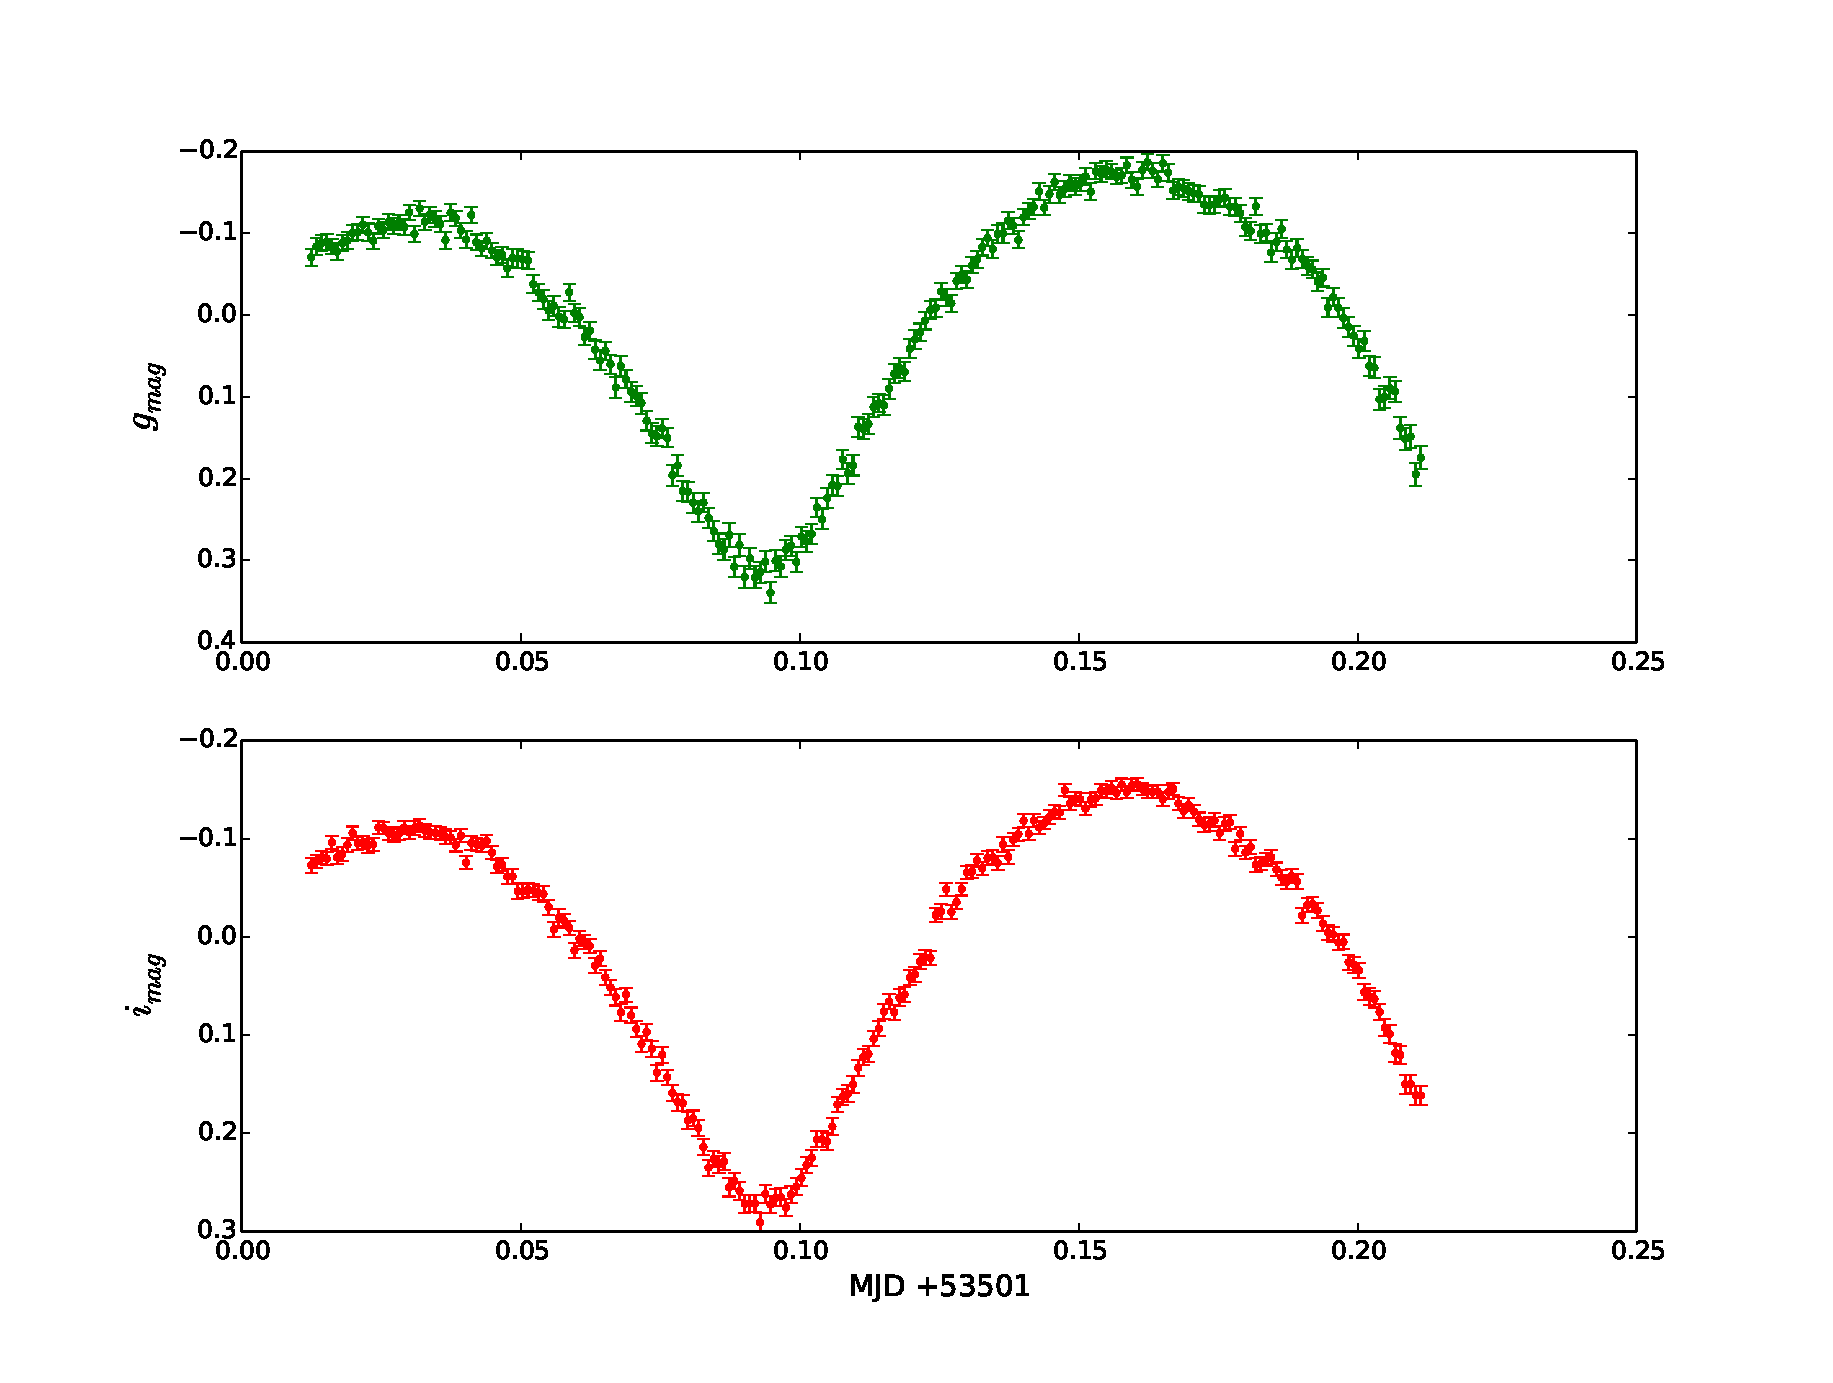
\includegraphics[width=120mm]{images/2005-05-10-run012-lightcurve-bin16.eps} 
    \caption{Sloan i and g light curves of object: 2005-05-10-run012-73. The data points are binned by a factor of 16. }
    \label{fig:2005-05-10-run012}
  \end{figure}
  
  \begin{figure}
    \center
    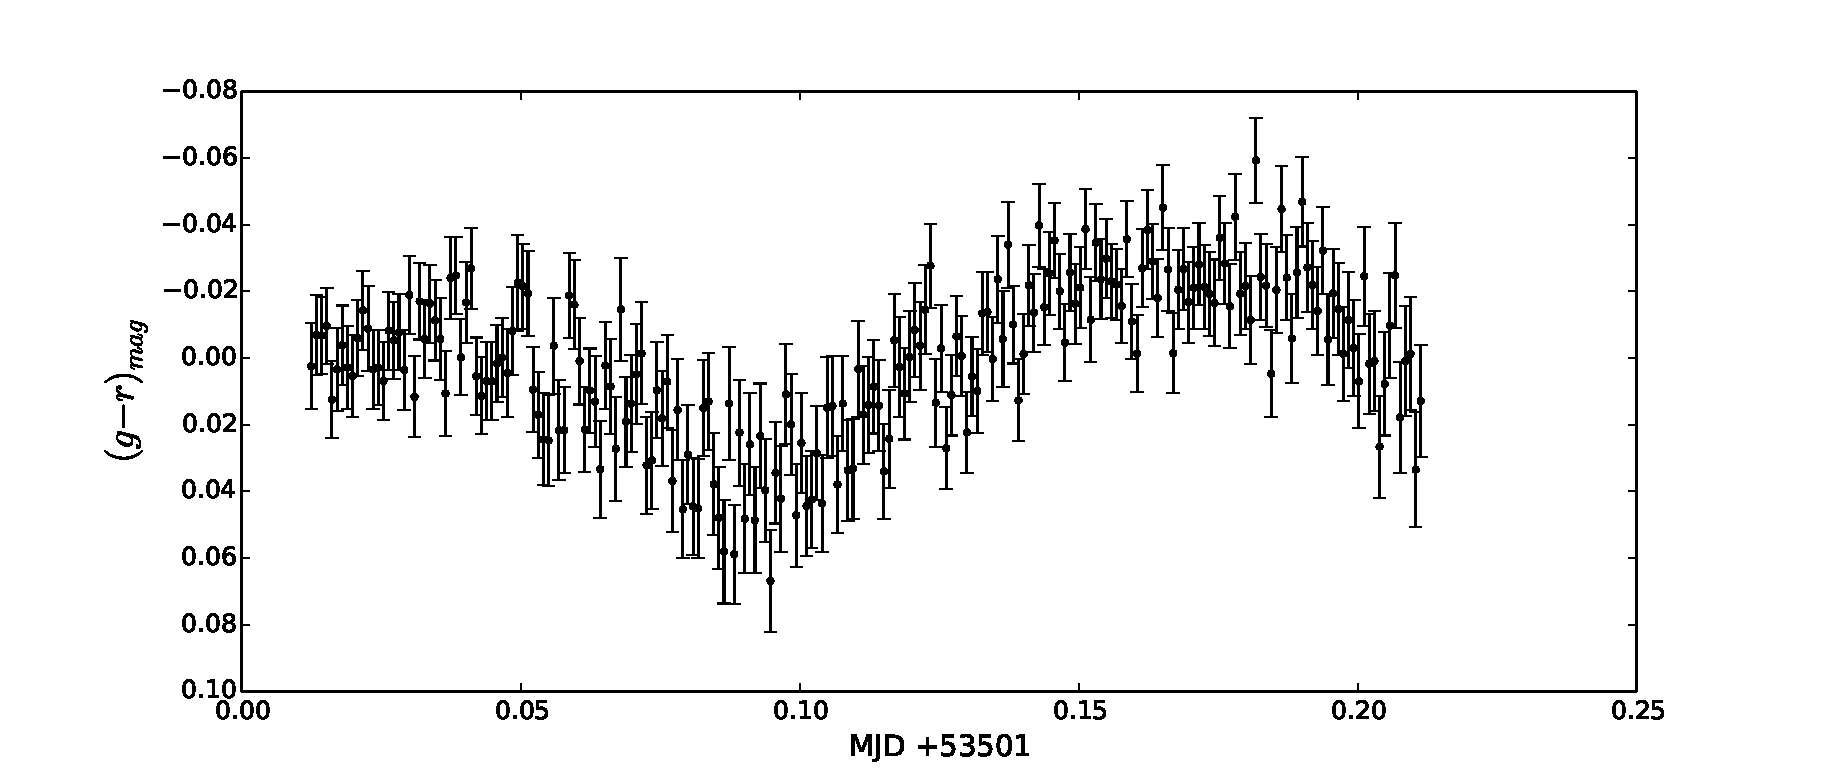
\includegraphics[width=120mm]{images/2005-05-10-run012-colourcurve-bin16.eps} 
    \caption{The $(g - i)$ colour light-curve of object: 2005-05-10-run012-73. The data points are binned by a factor of 16. }
    \label{fig:2005-05-10-run012-colour} 
  \end{figure}
  

  %Run date & 2005-05-10 \\
  %Pixel position & (232, 65) \\
  %URL: & \small \url{http://deneb.astro.warwick.ac.uk/phrnaw/sitedev/2005-05-10/run012.html} \\
  
The original target of this run was the X-ray transient, {GU Mus}, that was observed in quiescence in 2005. The compact object, thought to be a black hole, was accreting at the time and flickering is apparent in the optical light curve in all three of the Sloan i, g, and u bands, \citep{tariq2010}. About 4 arc minutes to the west we have detected a suspected {W UMa} contact binary with an apparent magnitude of $\sim21$ in Sloan g and period of $\sim 390$ minutes or 0.27 days. Visual inspection of the light-curves in figure \ref{fig:2005-05-10-run012} shows evidence of the O'Connell effect where the peak brightness of the second maximum is larger than the first. The object was too faint in the Sloan u band for us to produce any photometry. 

The cause of the O'Connell effect is something that is still under some debate. Differences in the depth of the minima of the light-curves is something that is expected and is caused by the different sizes and temperatures of each component in the system. Differences in the height of the maxima though is less obvious. Based on a geometric model of the eclipse though, we would expect the maxima to be of equal brightness. When the light-curve is at a maximum we are seeing the system side-on with the maximum area ellipsoidal faces presented to the observer. Current explanations for the O'Connell effect consist of star-spots that are locked in rotational synchronisation with the orbit and are presented preferentially on one side of the system; gas streams that create a hot-spot on or near one of the stars; and circumstellar material that is kinetically heated and gathered preferentially on the leading edge of the orbiting bodies, \citep{oconnelleffect}.  

In figure \ref{fig:2005-05-10-run012-colour} we plot the $(g-r)$ colour of the object. There is a clear modulation in the colour which must be due to temperature differences around the geometry of the system. The amplitude of this colour variation is $\Delta(g-r) = 0.06$ magnitudes. The minimum or coolest $(g - r)$ colour corresponds with the minimum of the light-curve. This is consistent with the idea that the hemispheres of the components in contact with each other are hotter due to a mutual reflection effect, while the outer hemispheres are cooler. The amplitude of the colour variation is $\Delta{(g-r)} \sim 0.06$ magnitudes.

% This target has another day of observations. 2005-05-09. The data should be combined, ephemeris found and light curve phase folded. 

\subsection{{W UMa}: 2013-07-21-run010-48}

\begin{figure}
  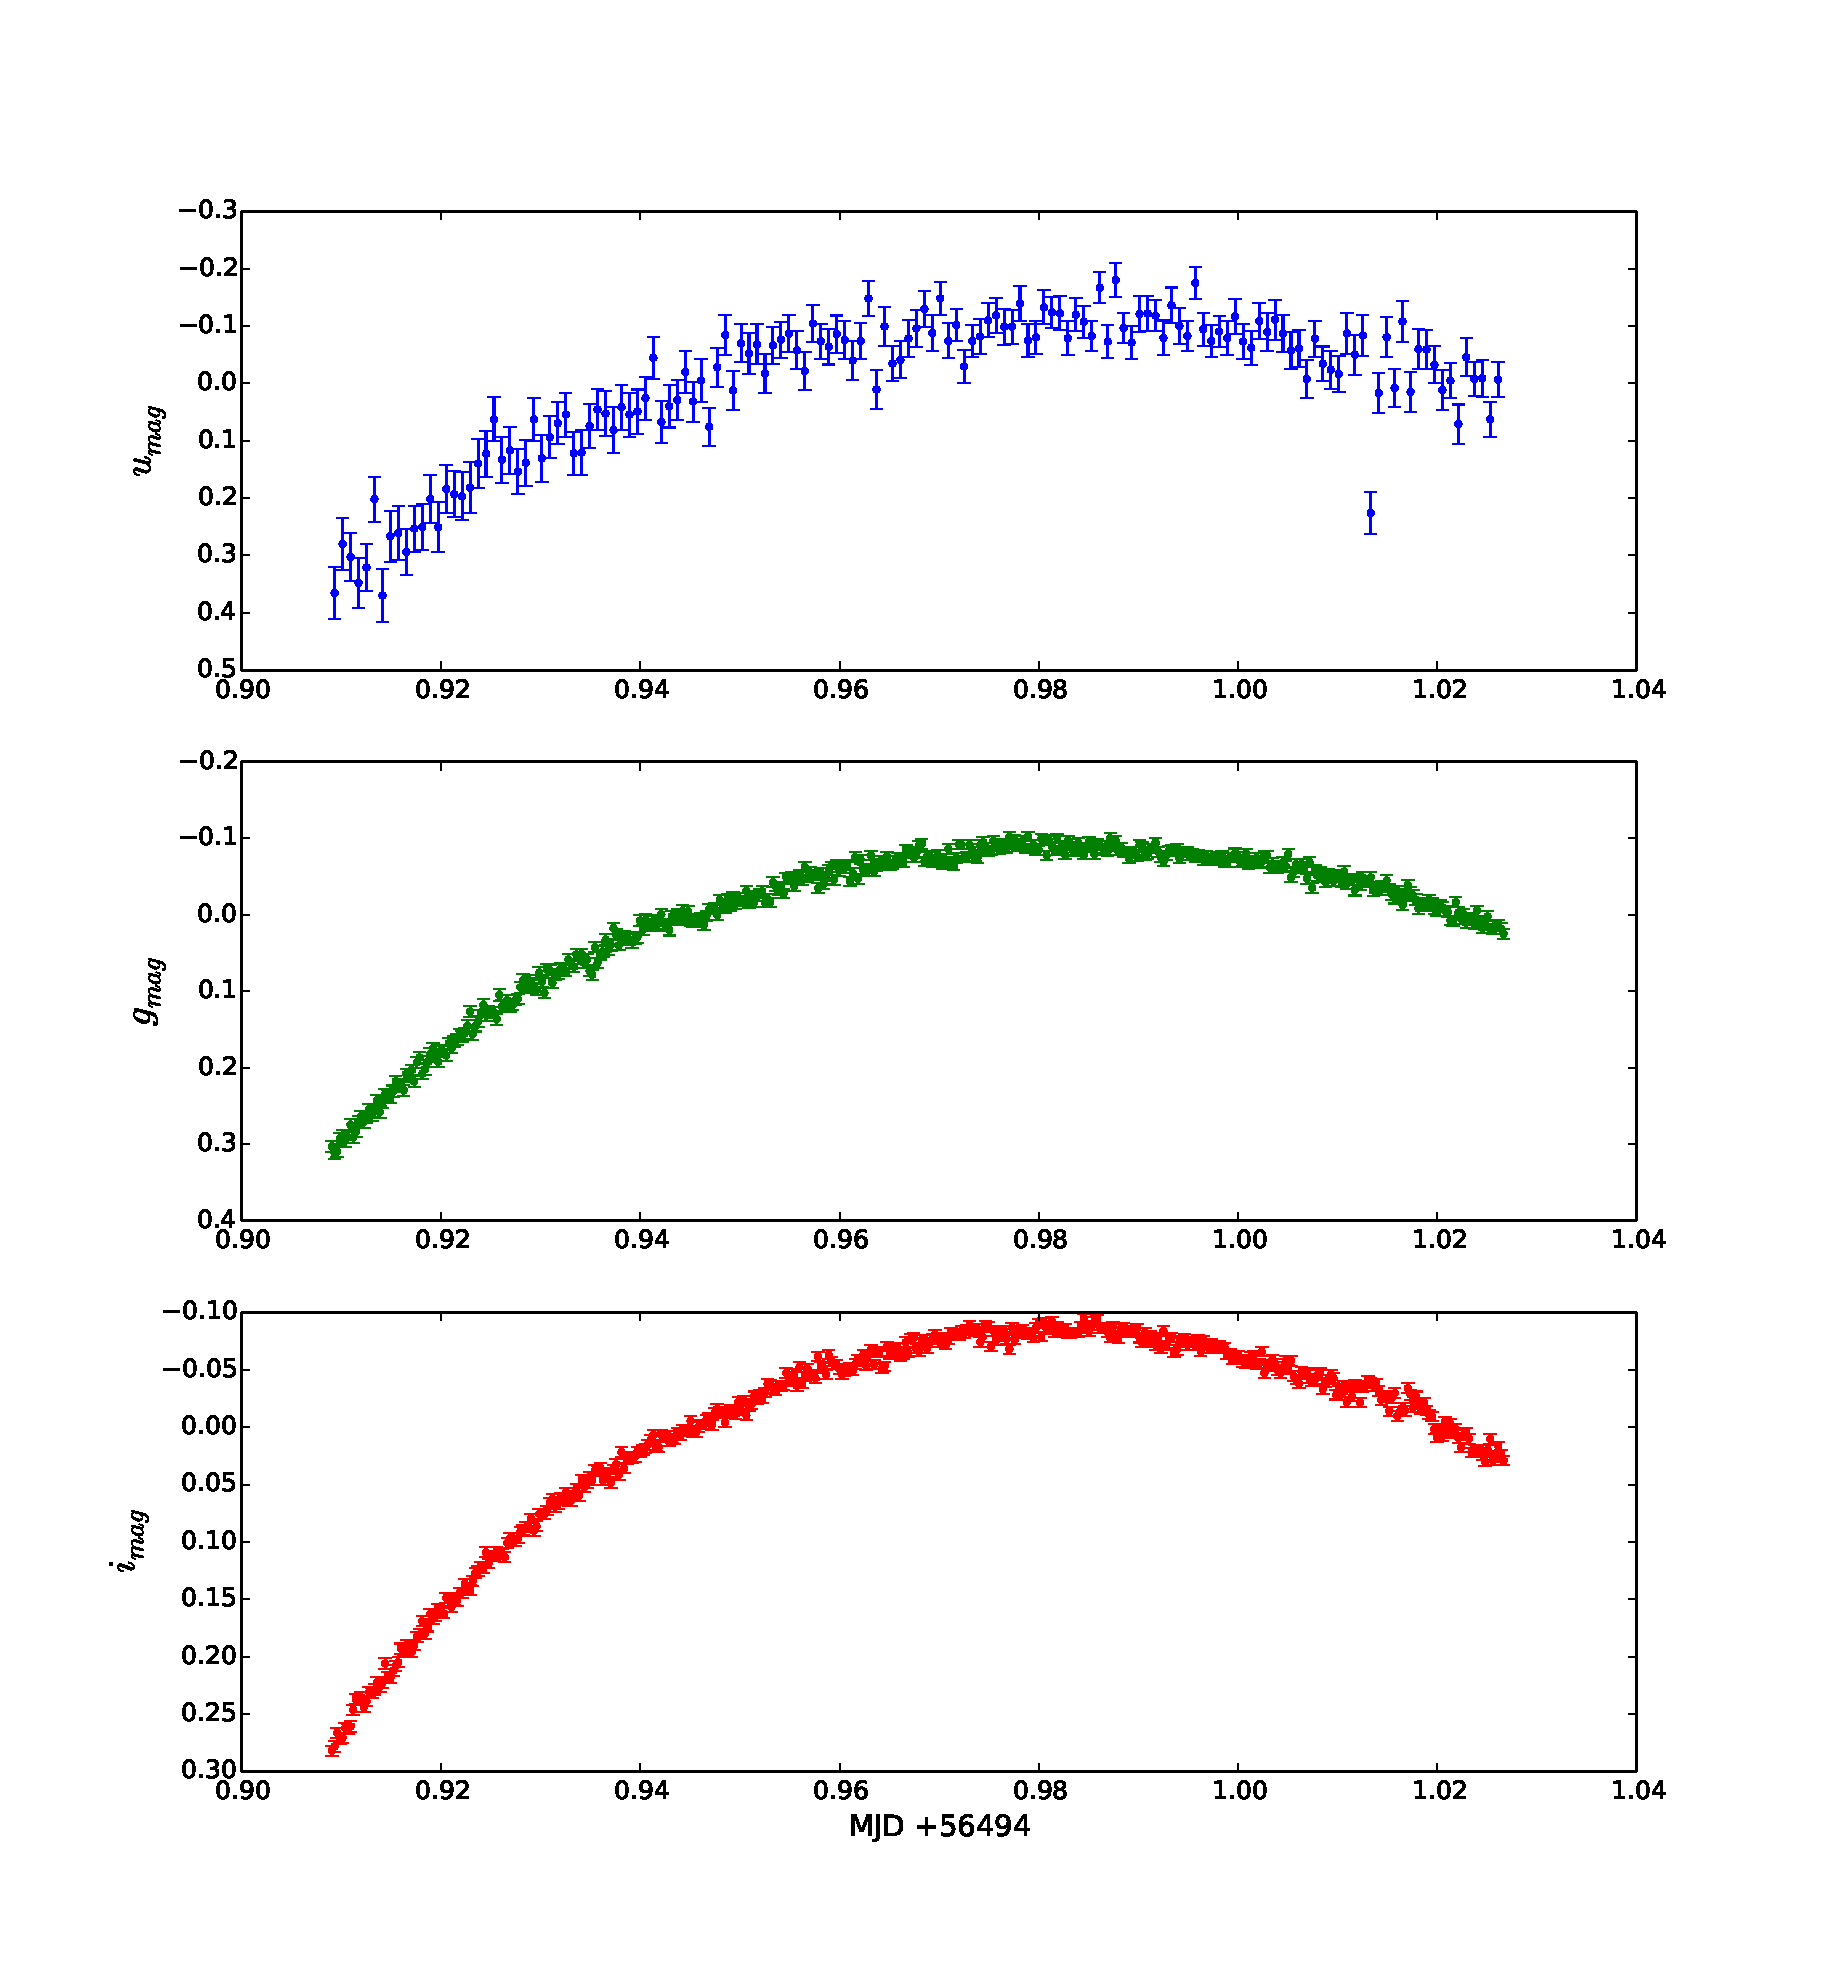
\includegraphics[width=120mm]{images/2013-07-21-run010-48_lightcurve-bin4.eps} 
  \caption{Sloan i, g and u light curves of object: 2013-07-21-run010-48. The data points are binned by a factor of 4.}
  \label{fig:2013-07-21-run010-48}
\end{figure}

\begin{figure}
  \center
  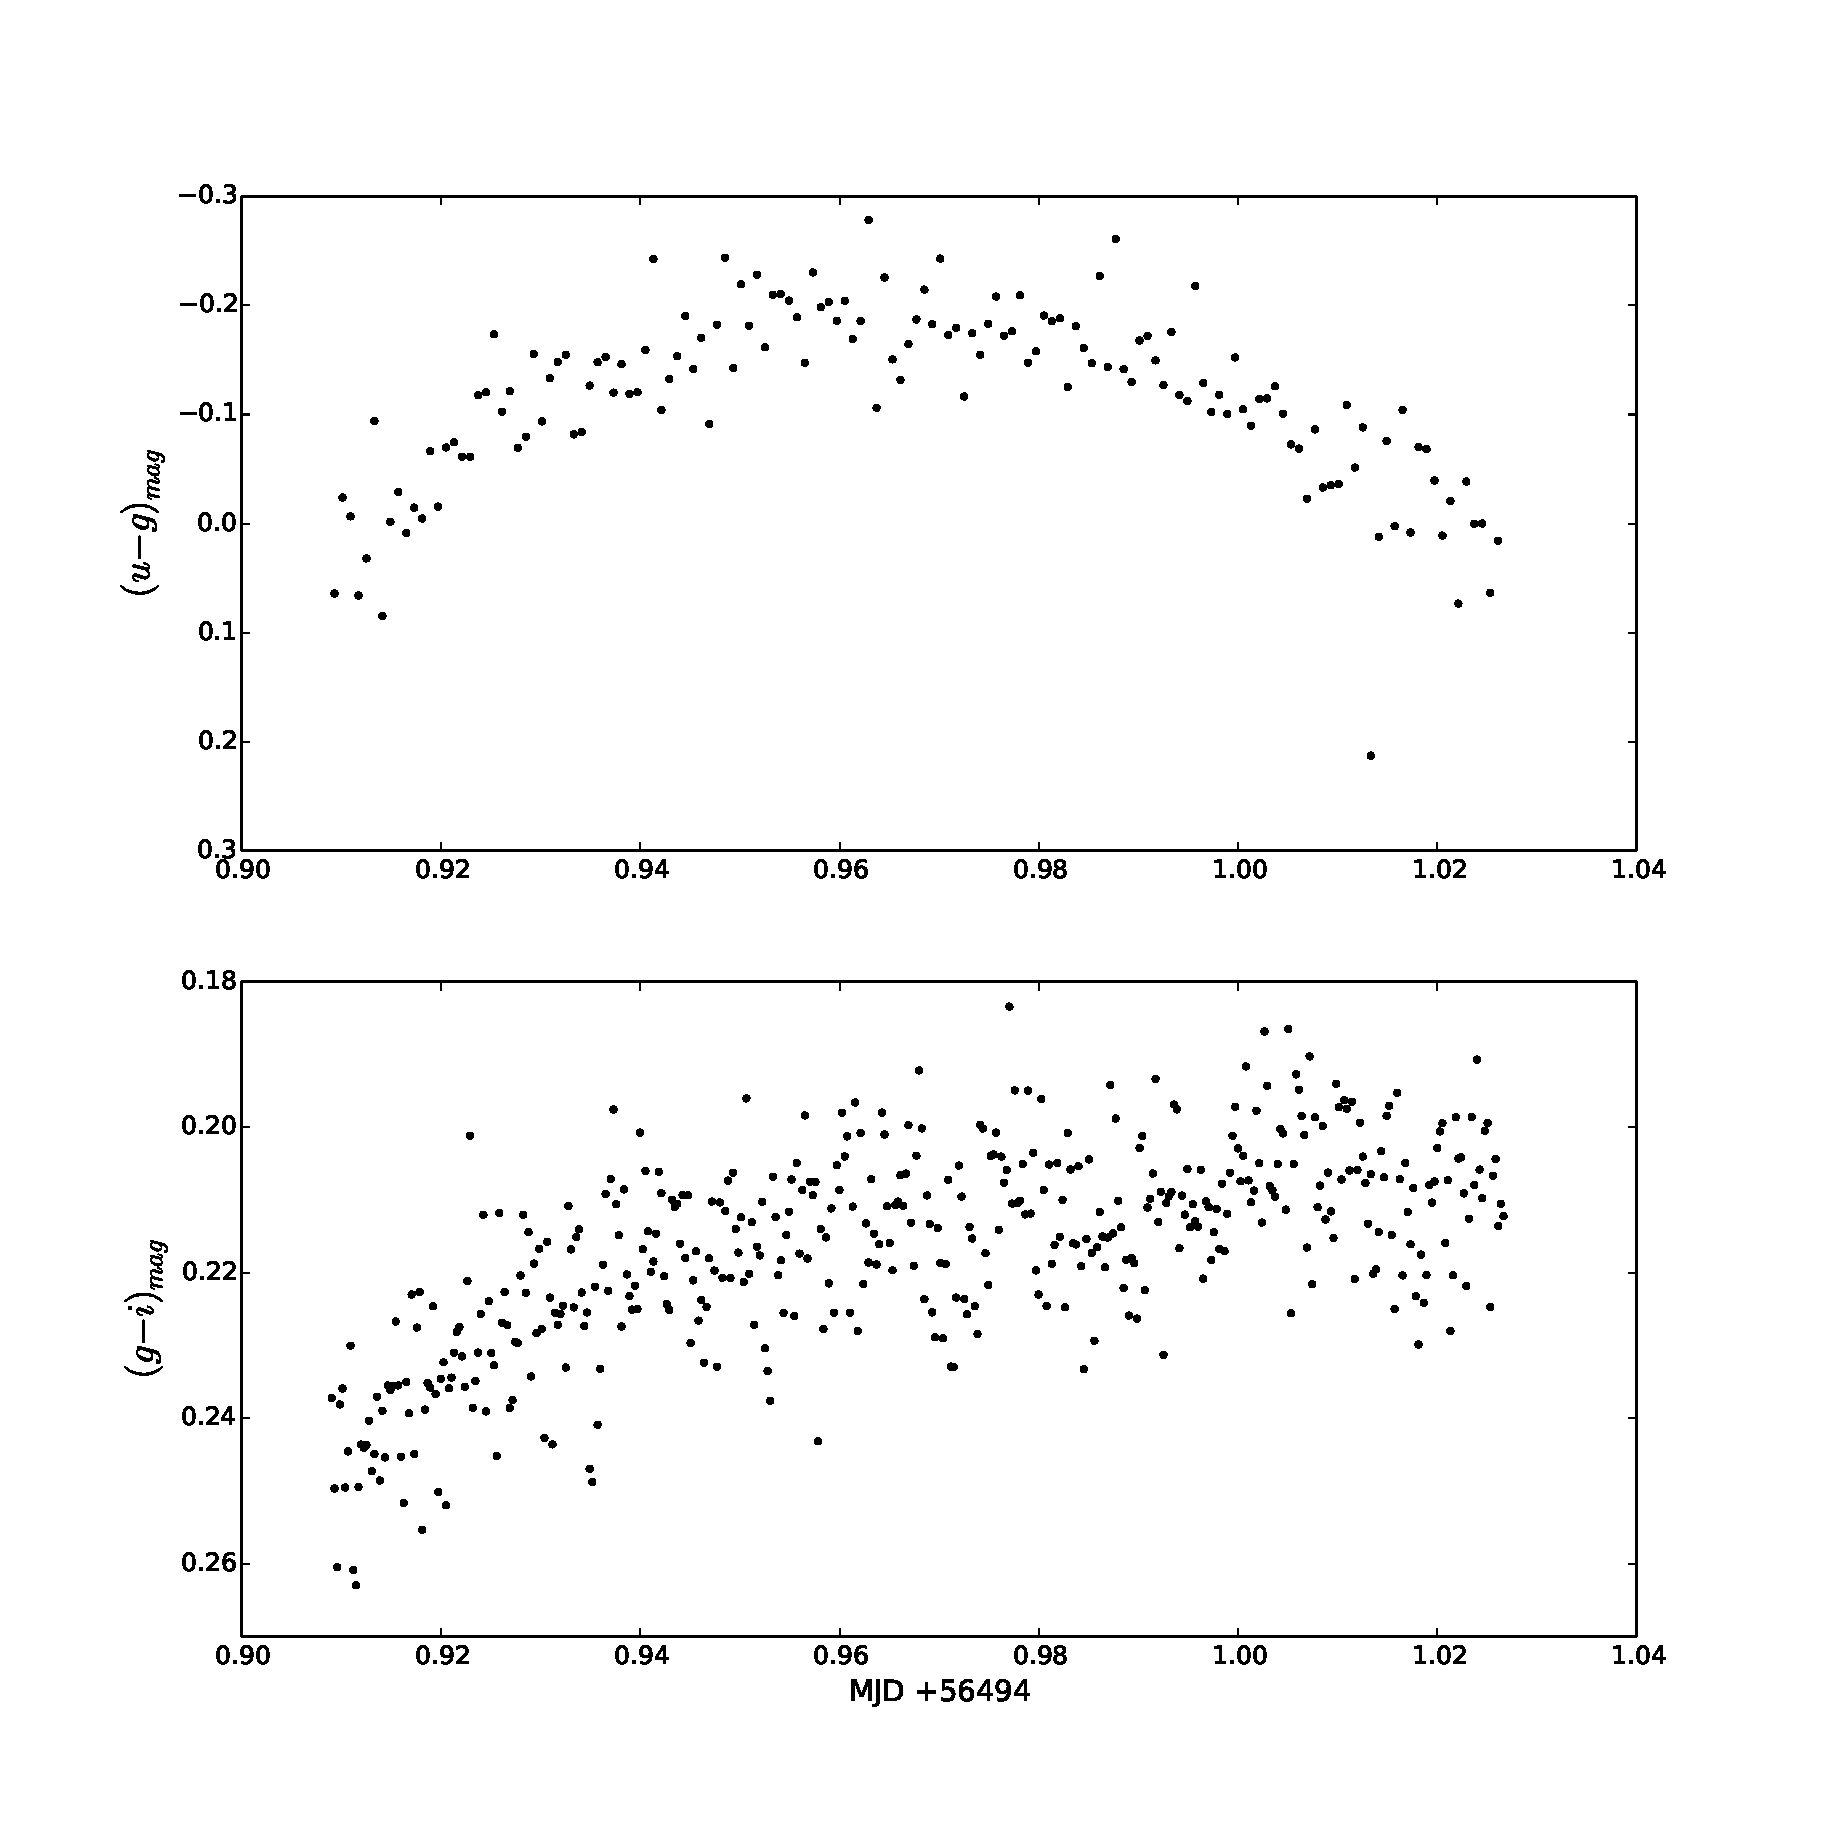
\includegraphics[width=120mm]{images/2013-07-21-run010-48_colourcurve-bin4.eps}
  \caption{Colour plots of $(u-g)$ and $(g-r)$ for object: 2013-07-21-run010-48. Data points are binned by a factor of 4.}
  \label{fig:2013-07-21-run010-48-colour}
\end{figure}


%  Classification & {W UMa} contact binary \\
%  ObjectID & 2013-07-21-run010-48 \\
%   Original target & J19440167+4017435 or KOI-823 \\
%   RA, DEC & 19:44:09.8, 40:16:34.4 (J2000) \\
%   Run date & 2013-07-21 \\
%   Pixel position & (452, 332) \\
 
This variable was the first one picked up by the automated pipeline and revealed itself during the very early development of the software. It appears on a relatively crowded Kepler field which has at least 5 newly discovered variable objects. Although this field has been monitored by the Kepler satellite, a search through the Kepler online archive \footnote{\url{https://archive.stsci.edu/kepler/data_search/search.php}} has not resulted in any data for this object. Since the aim of the Kepler mission is to discover exoplanets via observation of transits on stars that are relatively constant, it usually discards stars that are clearly variable. 

We suggest that this object is another {W UMa} category variable with an approximate period 400 minutes or 0.27 days. Unfortunately we do not have complete period coverage of the object's orbit and therefore this period is a very rough estimate. The target, KOI-823, has been observed with ULTRACAM on another occasion, 2013-07-28, but the field was set up differently (more to the west) and this object was not included. 

The colour plots for the object are shown in figure \ref{fig:2013-07-21-run010-48-colour}. As for the previous object, it seems that the $(g-i)$ colour peak coincides with the brightness maximum. However, it appears that the peak of the $(u-g)$ plot occurs significantly before the peak in brightness. \emph{Comment: Explanation for this?}


\subsection{{W UMa}: 2013-07-21-run010-163}

\begin{figure}
  \center
  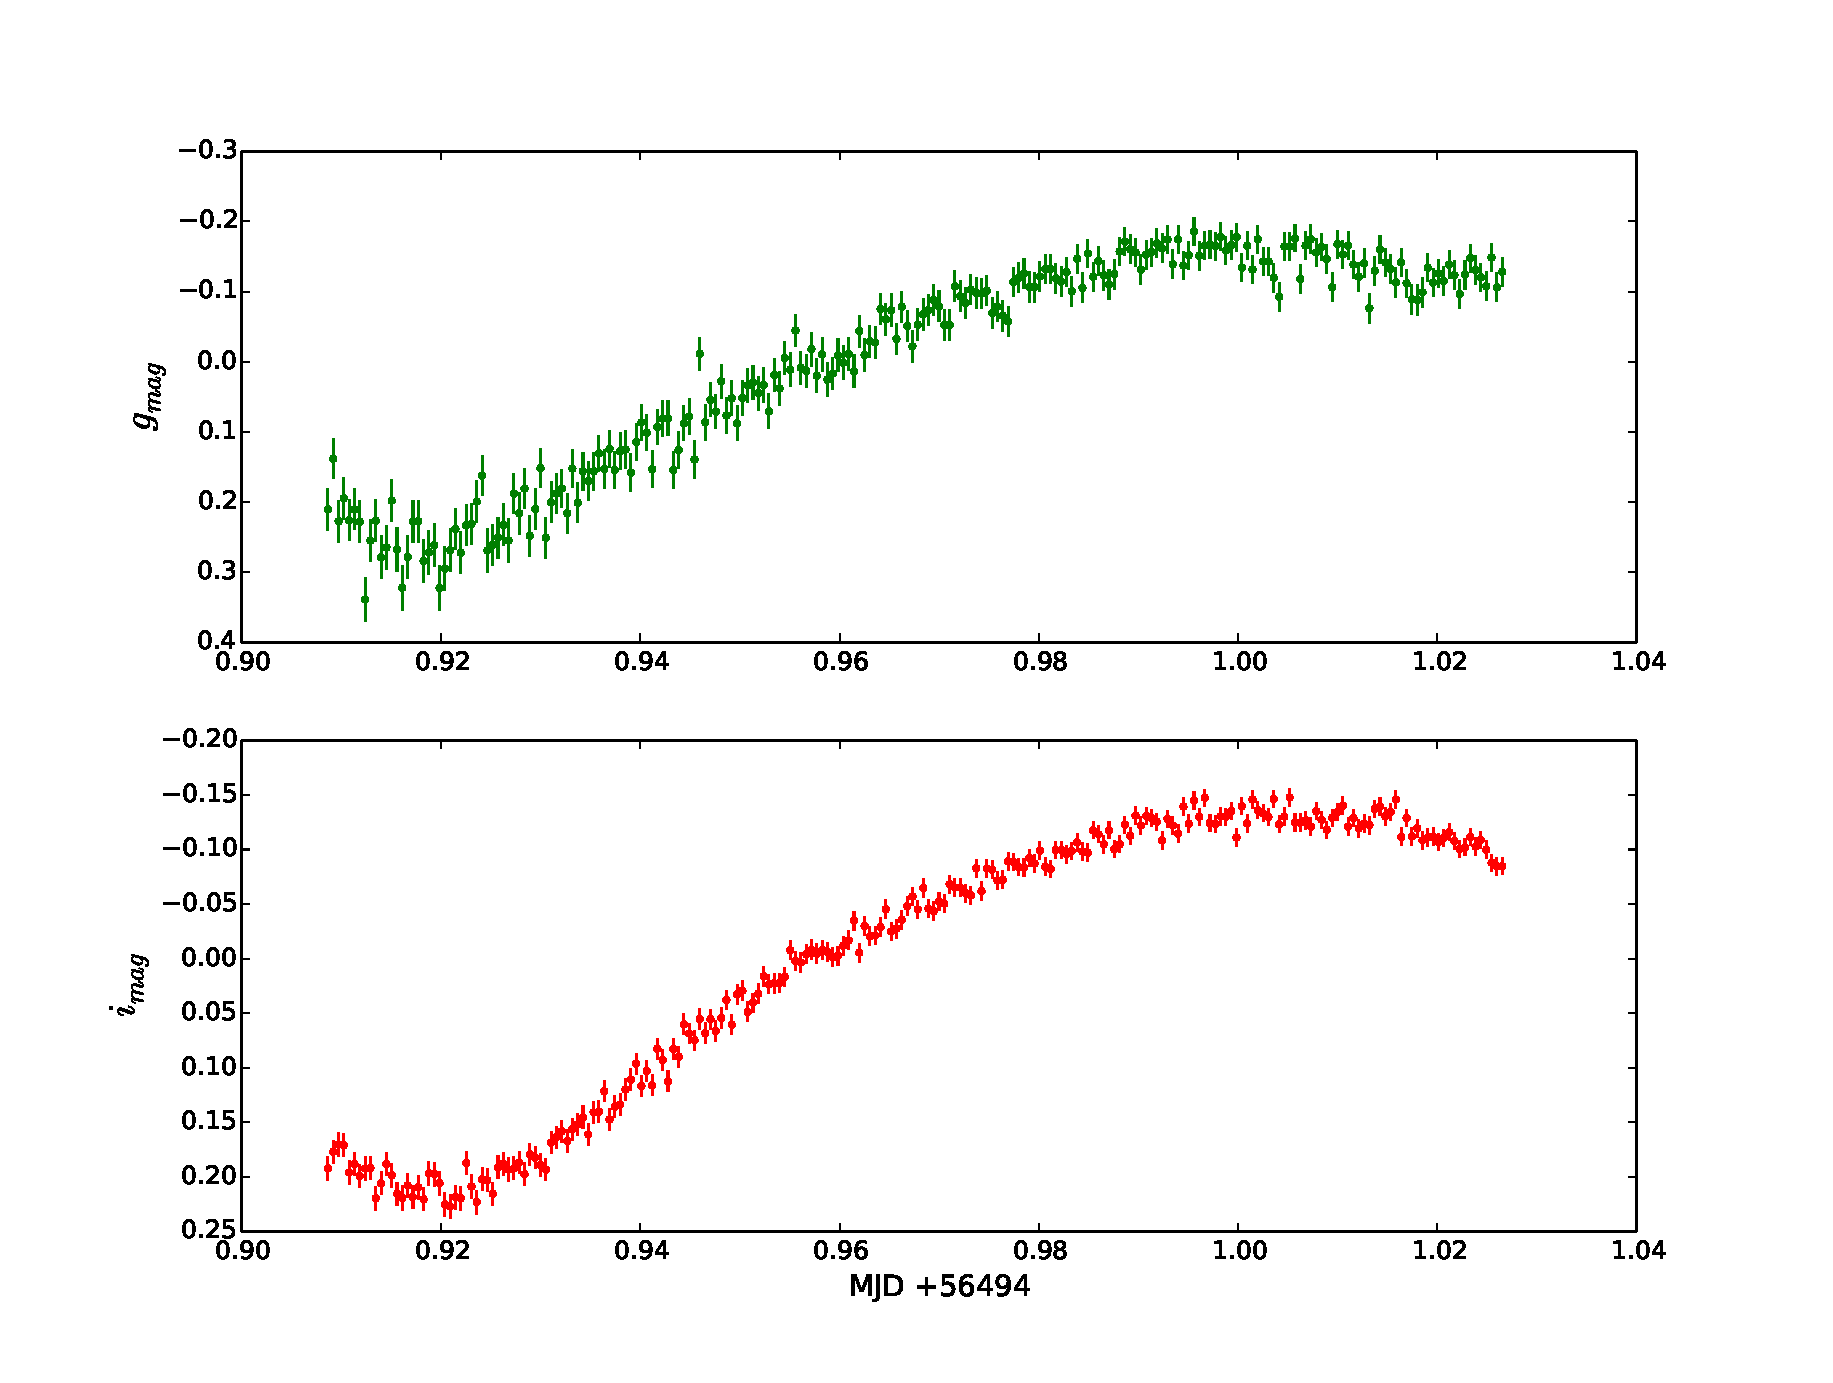
\includegraphics[width=120mm]{images/2013-07-21-run010-163_lightcurve-bin8.eps}
  \caption{Sloan i and g light curves of object: 2013-07-21-run010-163. Data points are binned by a factor of 8.}
  \label{fig:2013-07-21-run010-163}
\end{figure}

\begin{figure}
  \center
  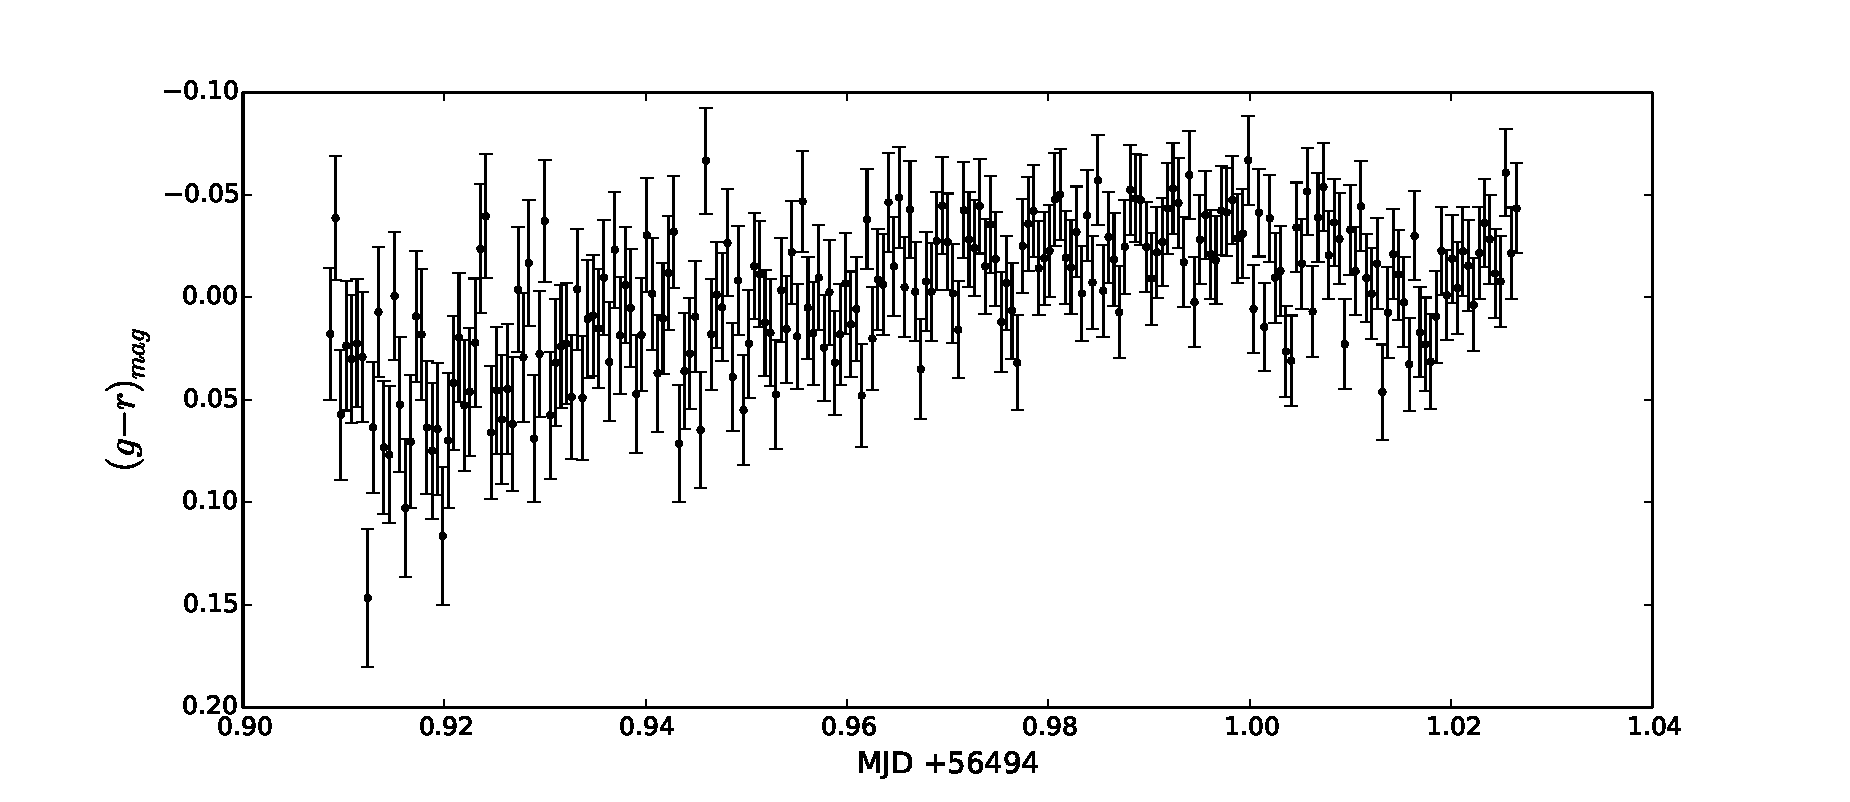
\includegraphics[width=120mm]{images/2013-07-21-run010-163_colourcurve-bin8.eps}
  \caption{The $(g - i)$ colour light-curve of object: 2013-07-21-run010-163. Data points are binned by a factor of 8.}
  \label{fig:2013-07-21-run010-163-colour}
\end{figure}


%   Classification & {W UMa} contact binary \\
%   ObjectID & 2013-07-21-run010-163 \\
%   Original target & J19440167+4017435 or KOI-823 \\
%   RA, DEC & 19:44:10.3, 40:18:08.1 (J2000) \\
%   Run date & 2013-07-21 \\
%   Pixel position & (417, 650) \\
  % URL: & \small \url{http://deneb.astro.warwick.ac.uk/phrnaw/sitedev/2013-07-21/run010.html} \\

This object is another suspected {W Uma} variable found on the same field as the previous object. The light-curve for this object includes one minimum and one maximum, although not a full orbit. From this light-curve we can estimate a period of about 460 minutes or 0.32 days.


\subsection{Eclipsing binary: 2013-07-21-run011-162}
  
\begin{figure}
  \center
  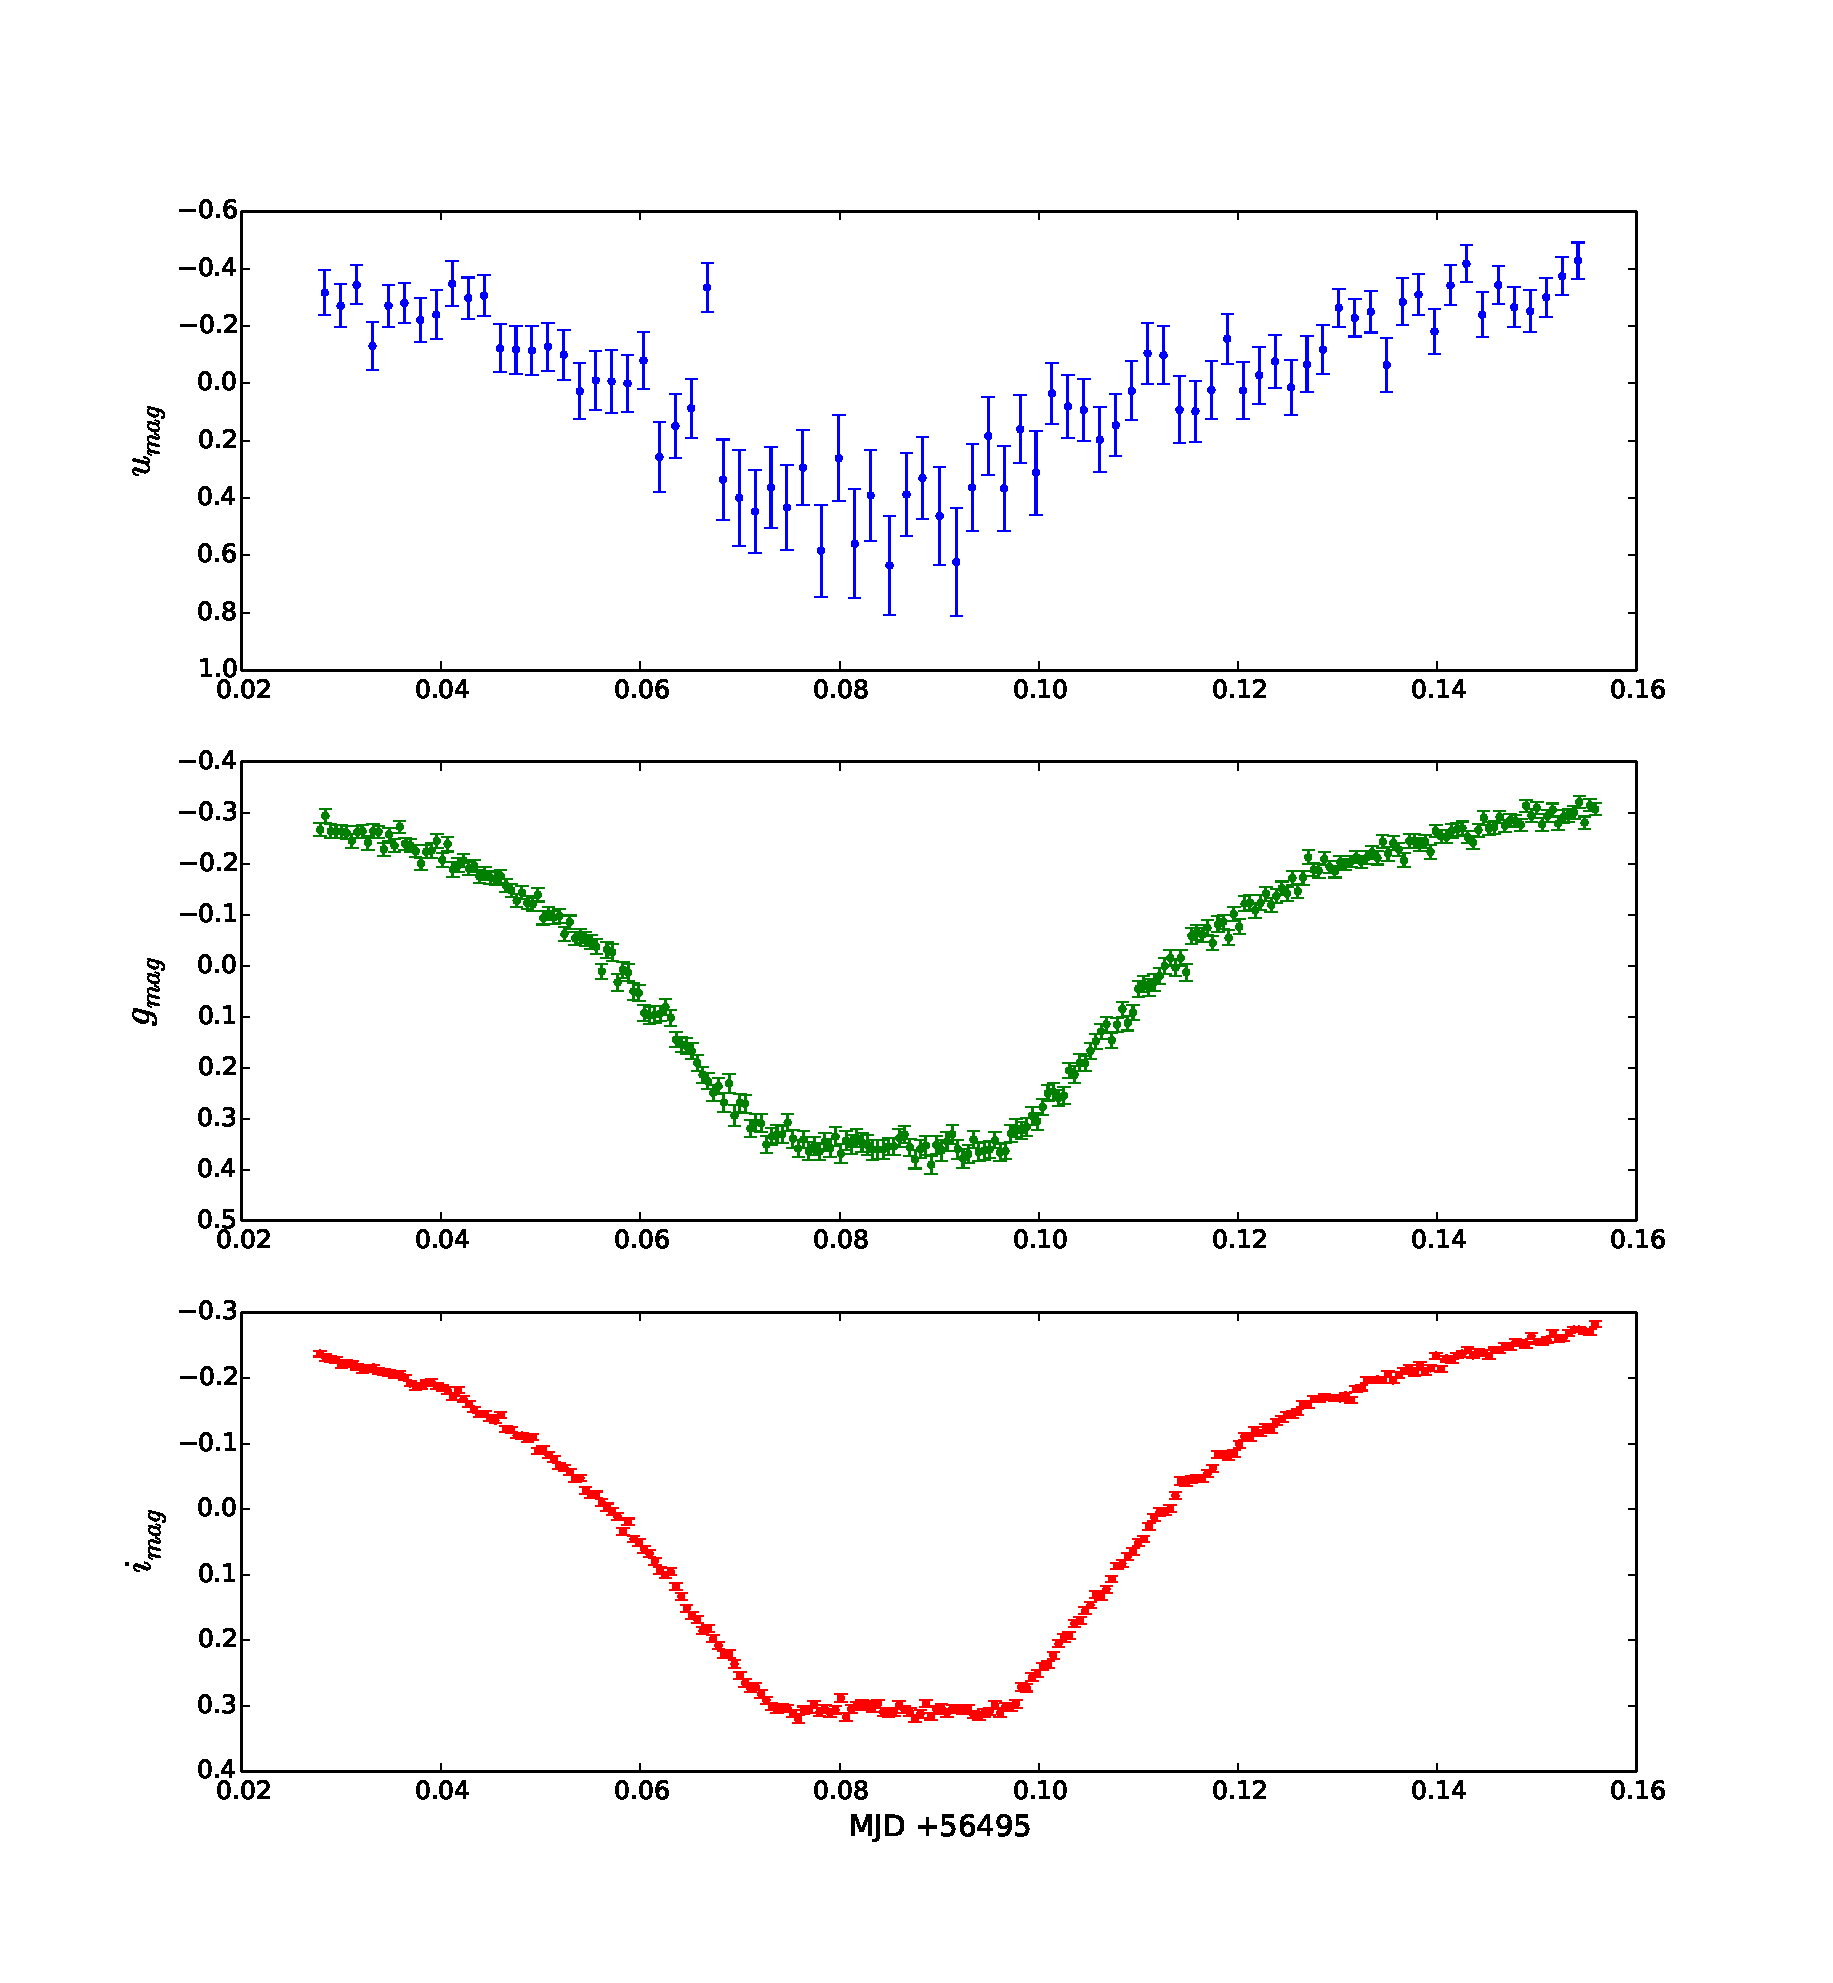
\includegraphics[width=120mm]{images/2013-07-21-run011-162_lightcurve-bin8.eps}
  \caption{Sloan i, g and u light curves of object: 2013-07-21-run011-162. Data points are binned by a factor of 8.}
  \label{fig:2013-07-21-run011-162}
\end{figure}

\begin{figure}
  \center
  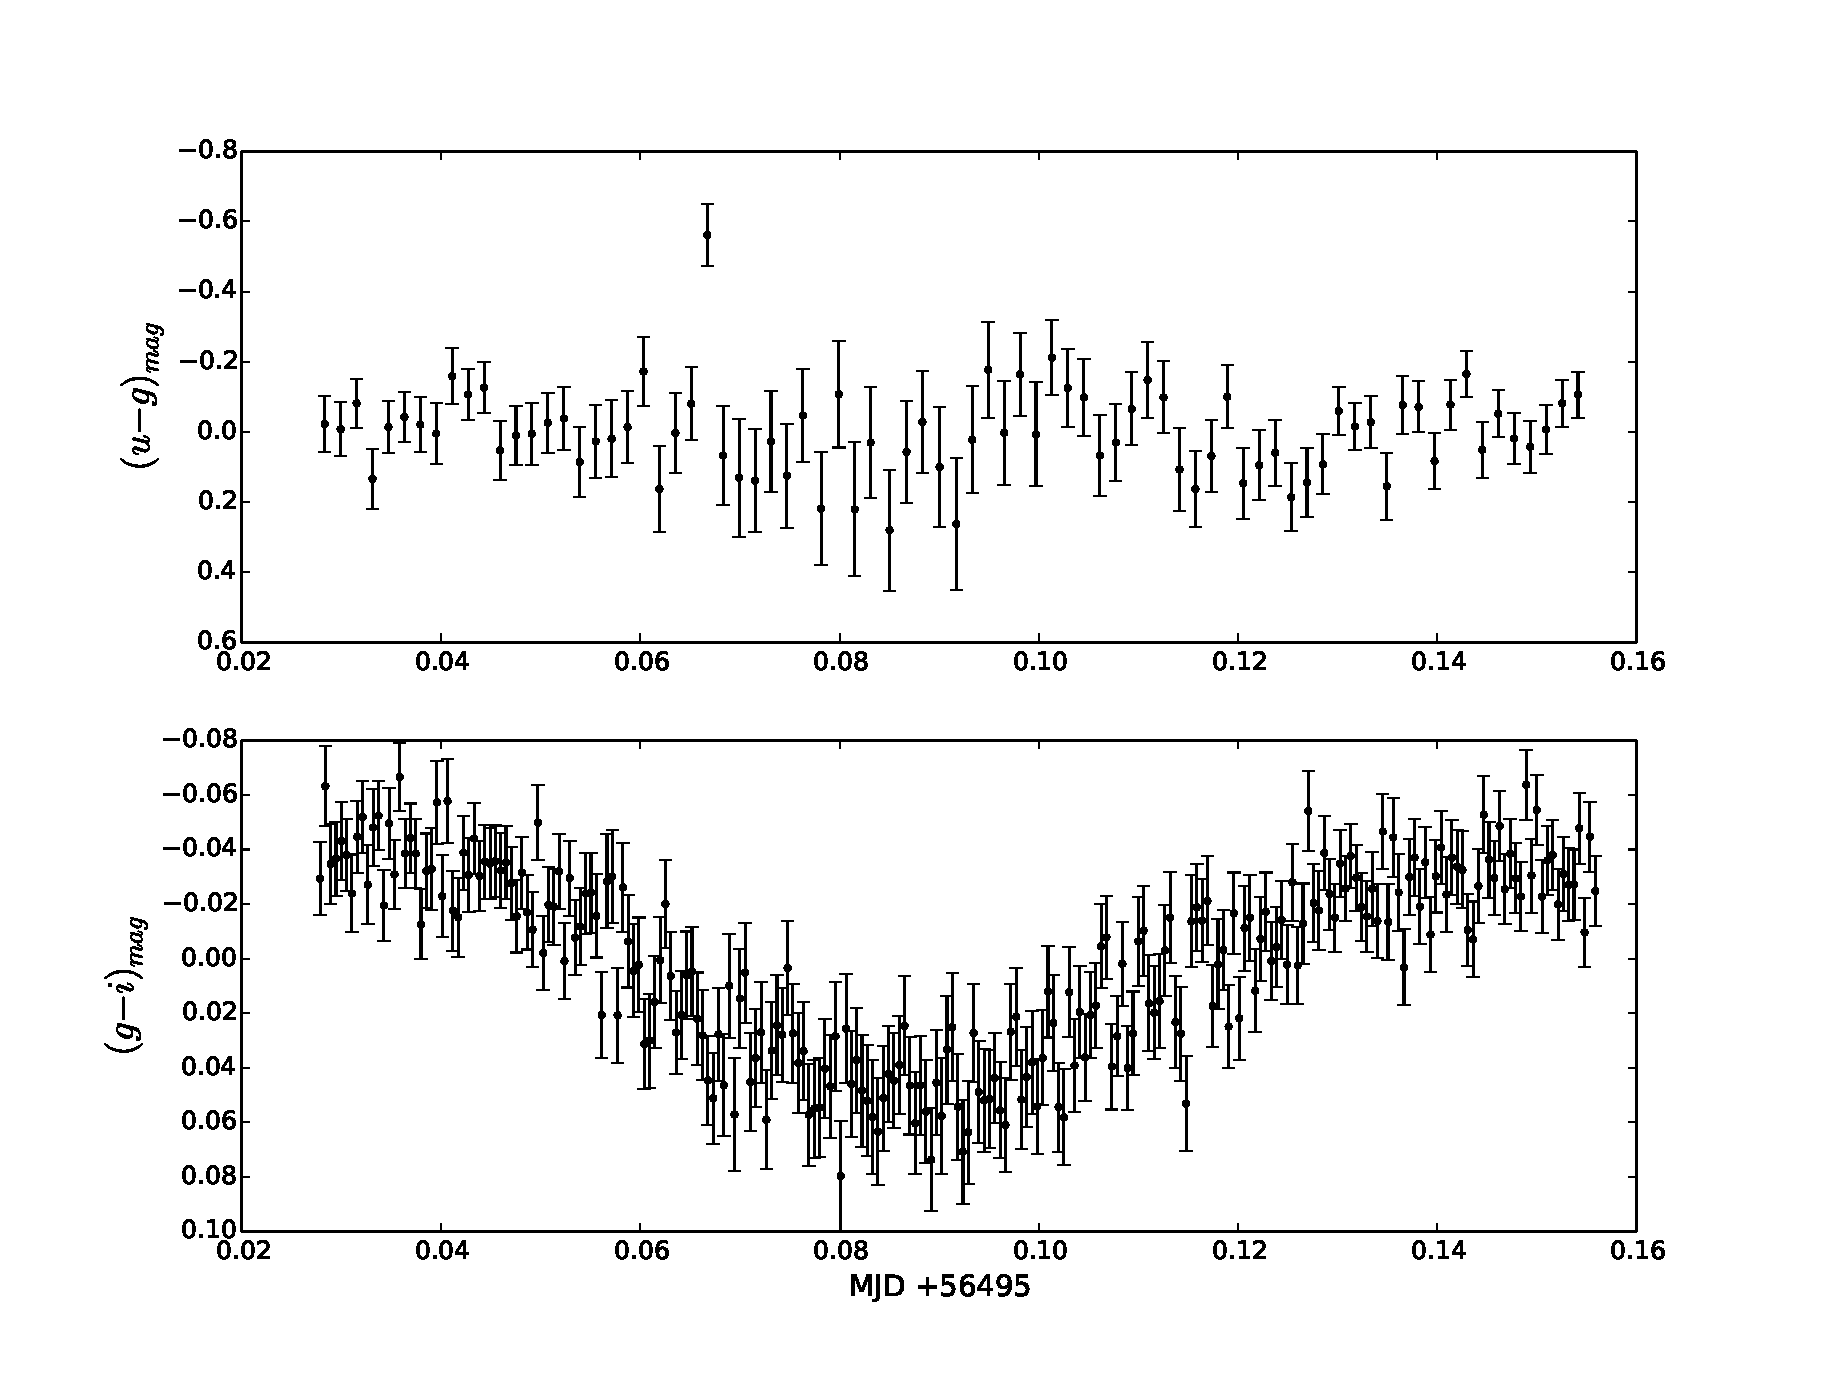
\includegraphics[width=120mm]{images/2013-07-21-run011-162_colourcurve-bin8.eps}
  \caption{$(u - g)$ and $(g - i)$ plots for the object: 2013-07-21-run011-162. Data points are binned by a factor of 8.}
  \label{fig:2013-07-21-run011-162-colour}
\end{figure} 


%   Classification & Eclipsing binary \\
%   ObjectID & 2013-07-21-run011-162 \\
%   Original target & 2MASS J19540329+403822 or KOI-1546 \\
%   Pixel position & (726, 341) \\
%   RA, DEC & 19:54:01.7, 40:37:34 (J2000) \\
%   URL: \url{http://deneb.astro.warwick.ac.uk/phrnaw/sitedev/2013-07-21/run011.html} \\

The light curve of this object includes a primary eclipse. Since the eclipse profile has a 'flat-bottom' we can conclude that this eclipse is total (ie that the primary is completely obscured by the secondary during the eclipse. This also means that the primary has a smaller diameter than the secondary. The primary eclipse duration is 37 minutes. The depth of the eclipse is about 0.7 magnitudes which corresponds to a drop in flux of 50\%. 

It is notable that the ingress and the egress demonstrates broad `wings' suggesting that the object being eclipsed (primary) is extended and the shape of the curve suggests tidal distortion of the secondary. The colour plots in figure \ref{fig:2013-07-21-run011-162-colour} show that the minimum of the $(g-i)$ coincides with the center of the eclipse. The colour plots do not show the clear flat-bottom that we see in the light-curves for $i$ and $g$. 

Although the object is in a Kepler field and is, in fact, close to KOI-1546, a search through the Kepler archive \footnote{\url{https://archive.stsci.edu/kepler/data_search/search.php}} reveals that it is not listed. 



\subsection{$\delta$ Scuti: 2013-07-21-run010-23}

\begin{figure}
  \center
  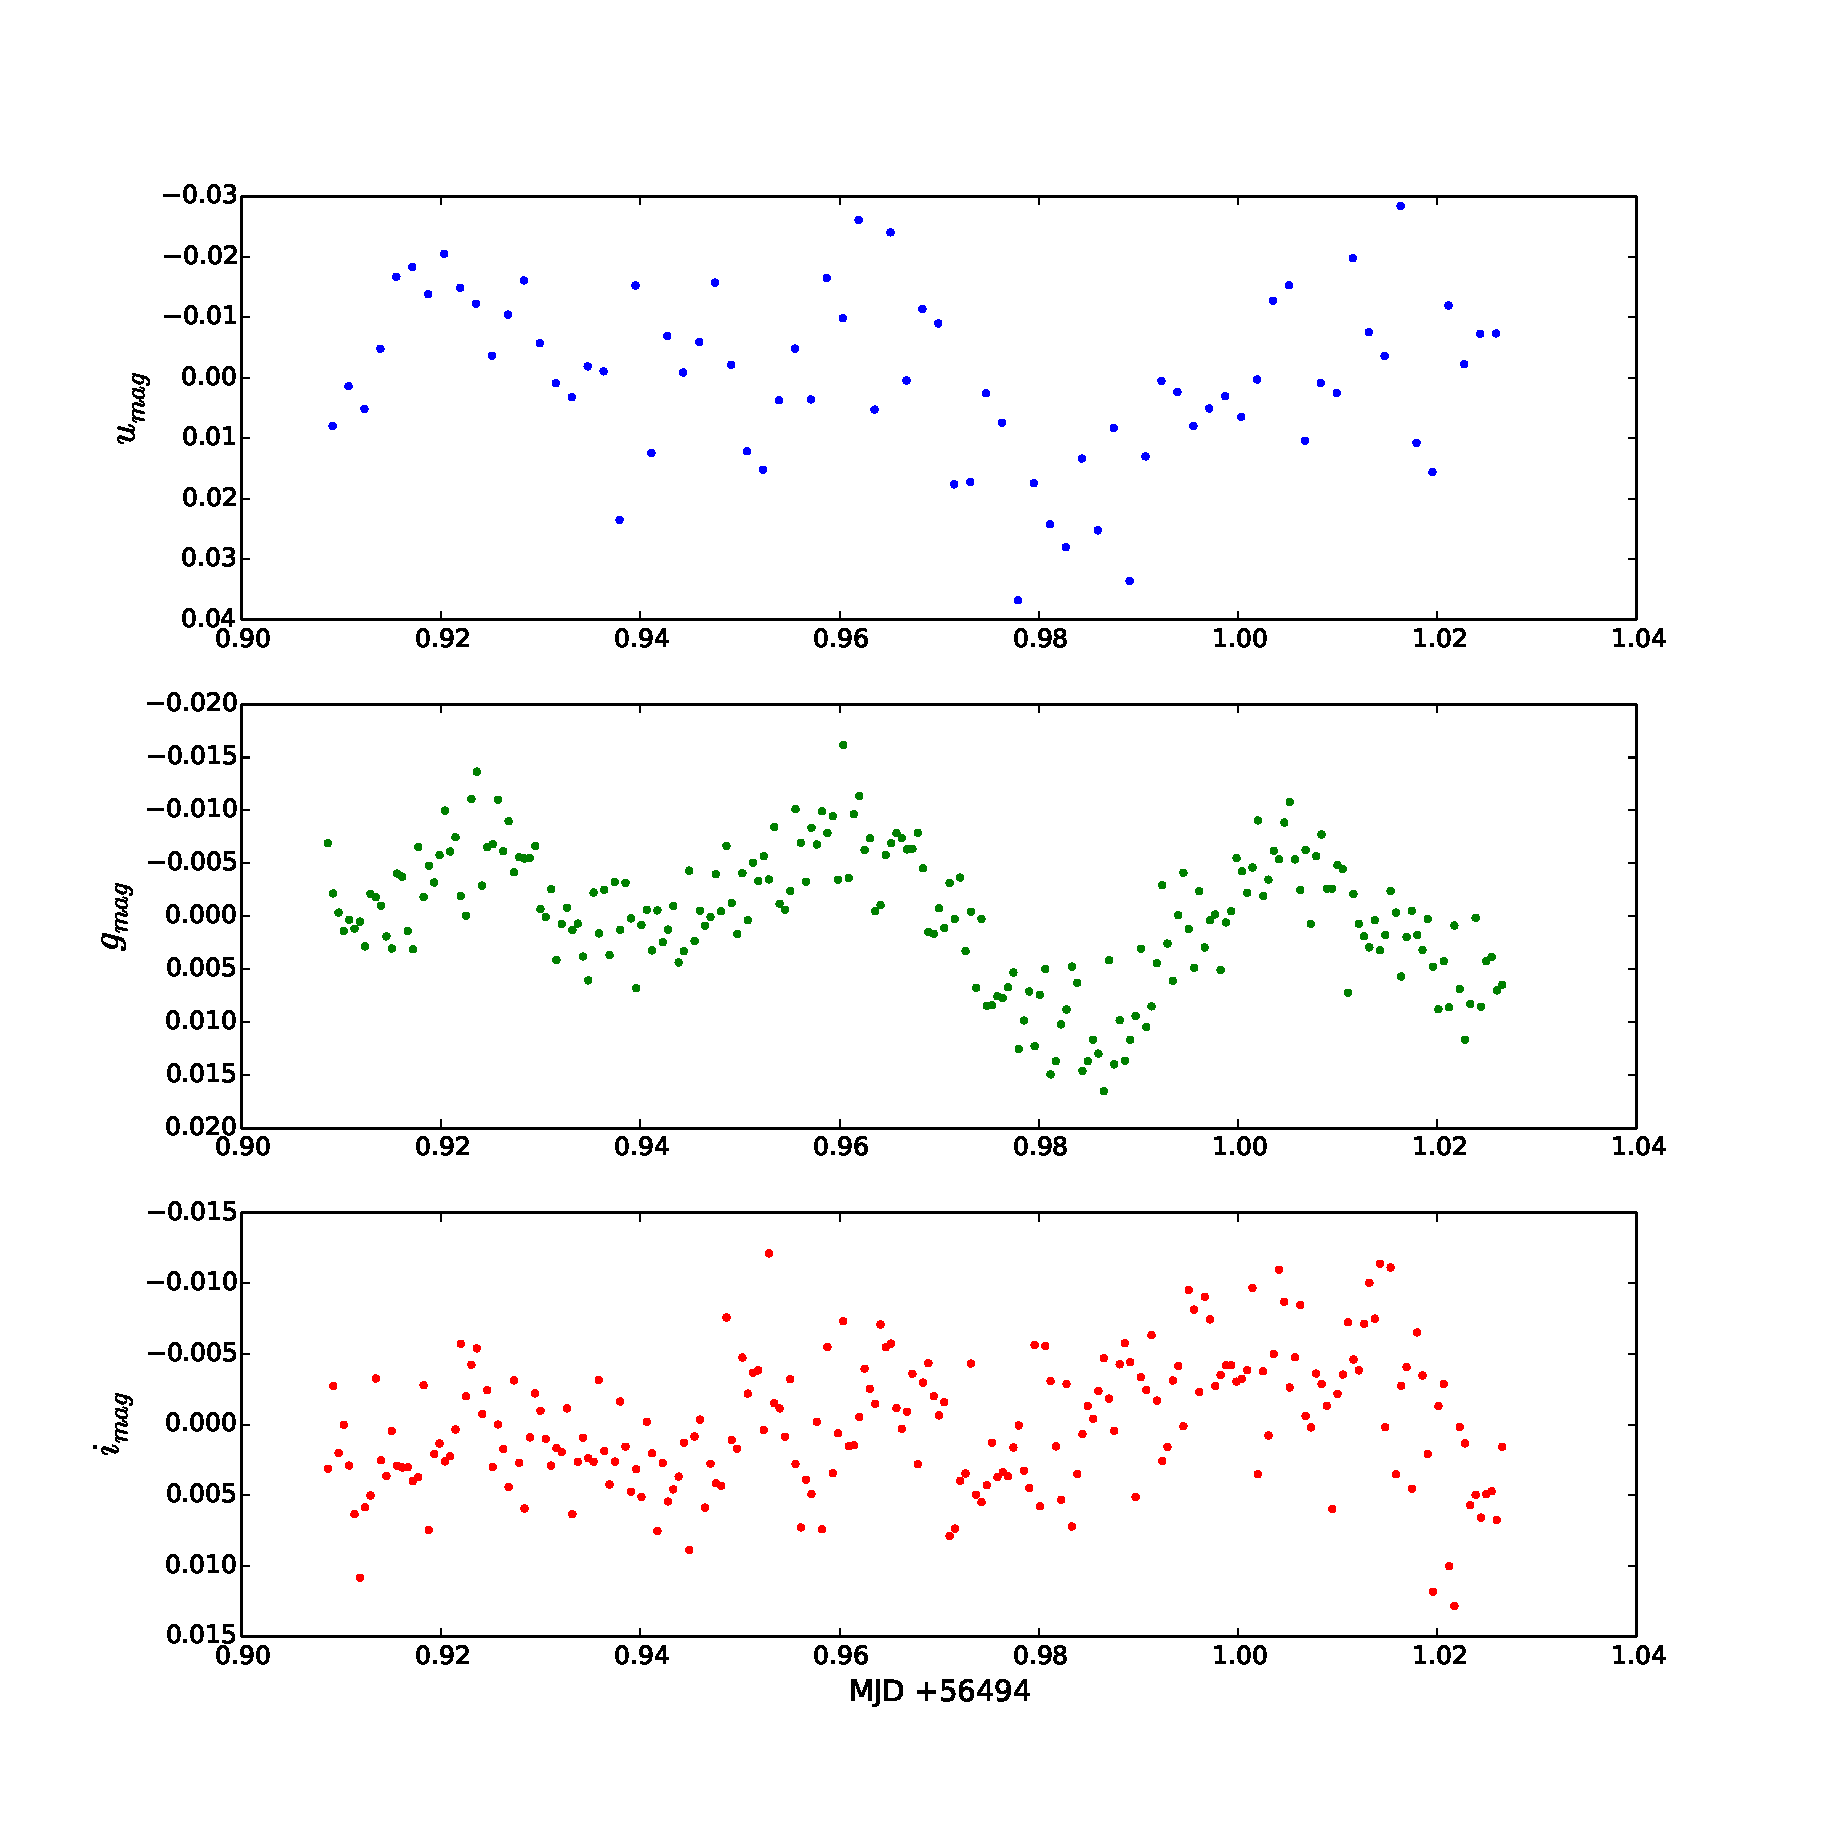
\includegraphics[width=120mm]{images/2013-07-21-run010-23_lightcurve-bin8.eps} \\
  \caption{Sloan i, g and u light curves of object: 2013-07-21-run010-23. Data points are binned by a factor of 8.}
  \label{fig:2013-07-21-run010-23}
\end{figure}

\begin{figure}
  \center
  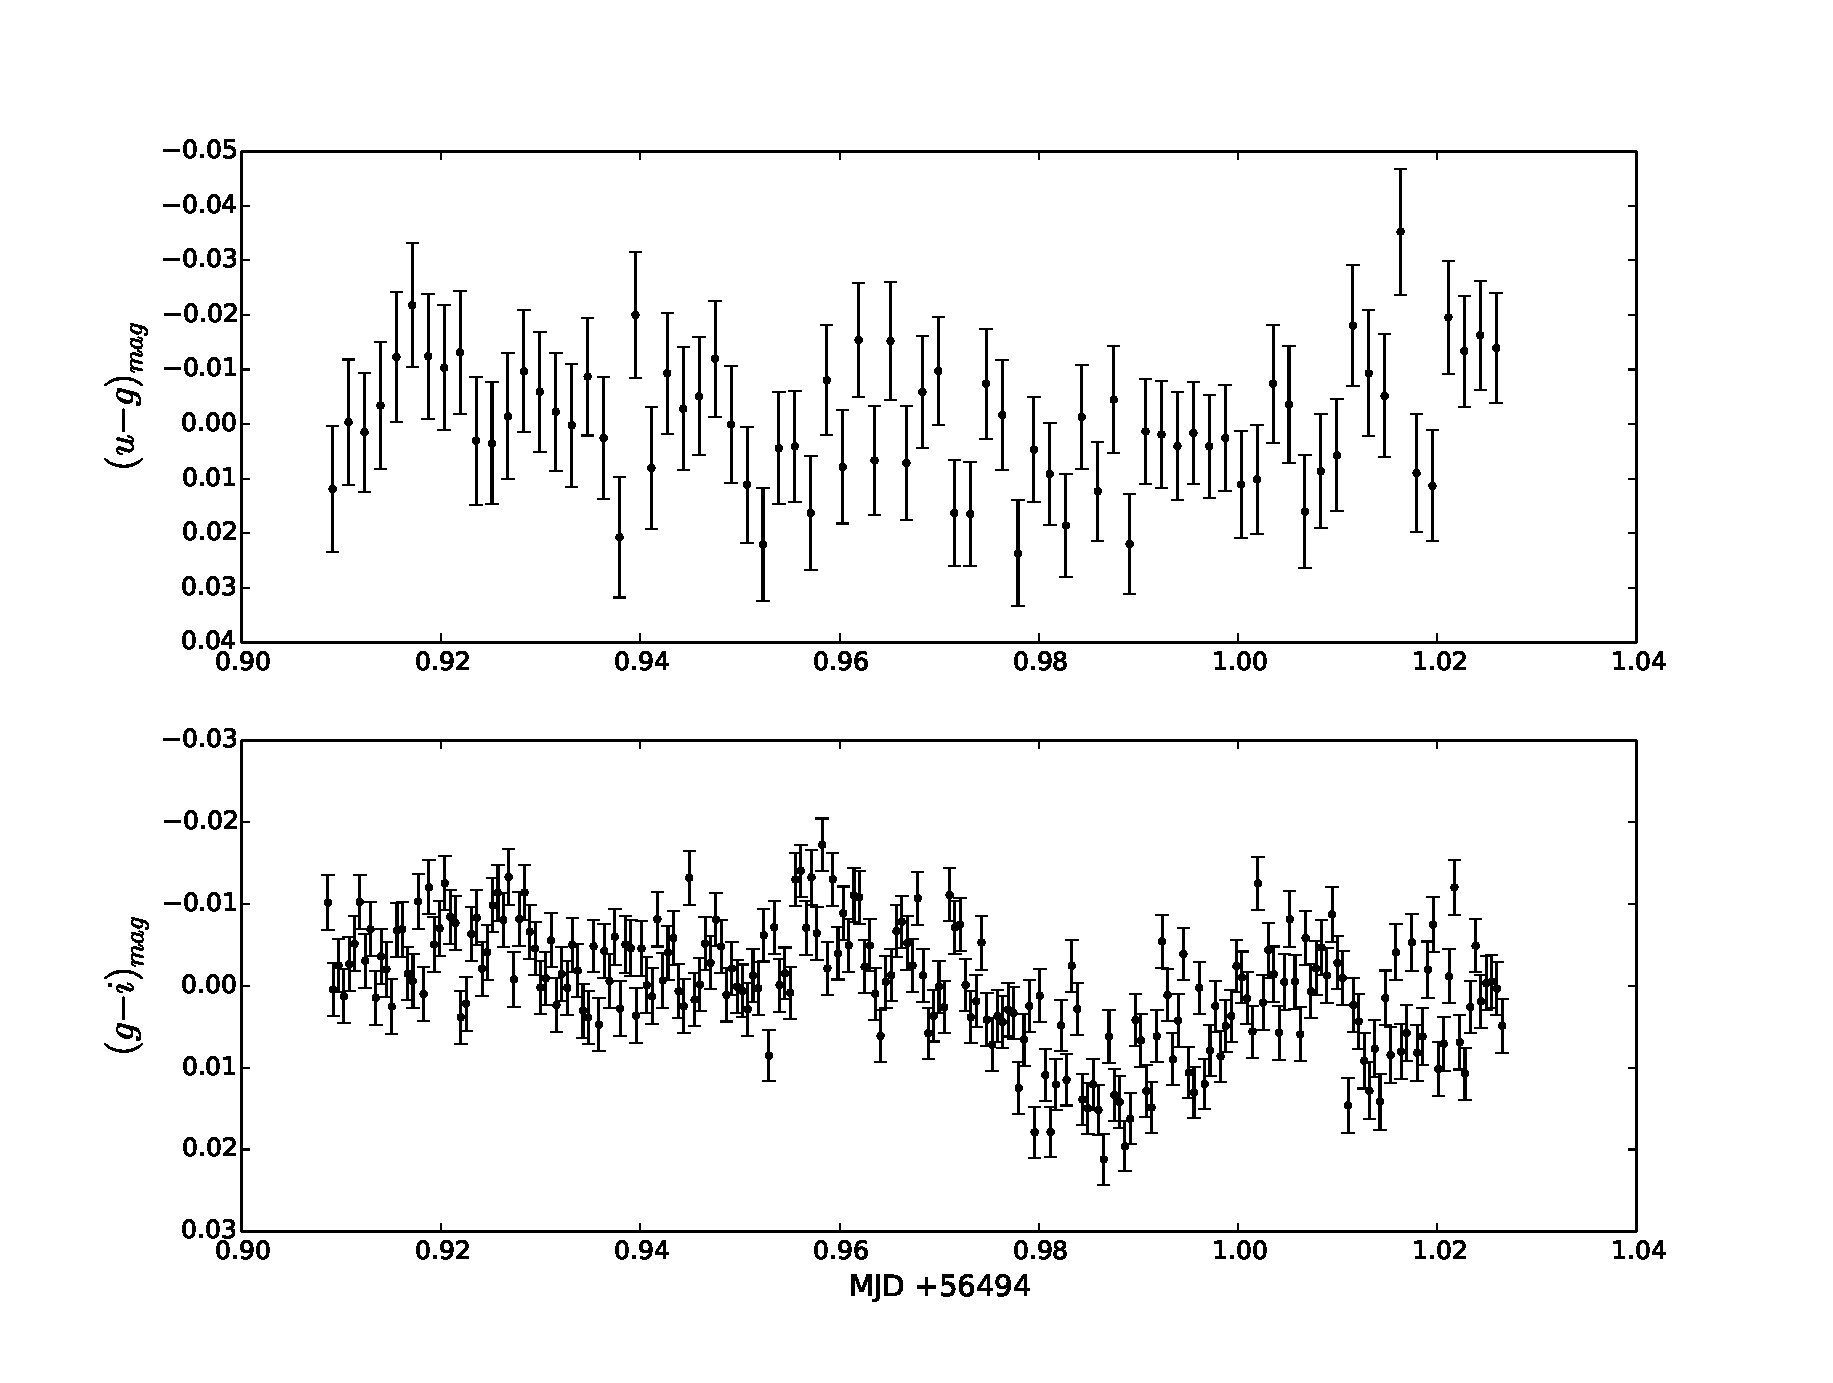
\includegraphics[width=120mm]{images/2013-07-21-run010-23_colourcurve-bin8.eps} \\
  \caption{$(u - g)$ and $(g - i)$ plots for the object: 2013-07-21-run010-23. Data points are binned by a factor of 8.}
  \label{fig:2013-07-21-run010-23-colour}
\end{figure}



%   Classification & $\delta$ Scuti \\
%   ObjectID & 2013-07-21-run010-23 \\
%   Original target & J19440167+4017435 or KIC5115978 \\
%   Pixel position & (54, 362) \\
%   RA, DEC & 19:44:19.6, 40:16:43.7 (J2000) \\

This object was found on a run that included the exoplanet host, KIC5115978, which has at least one planet, \citep{KIC5115978}. The new variable is located about 6 arc minutes away from the target. A search of the Kepler data archive \footnote{\url{http://archive.stsci.edu/kepler/kepler_fov/search.php}} gives no results for this object. Unfortunately this object is not in the Kepler field of view, but lies in a position that does not fall on the Kepler CCD. We have no further photometry for this object. 

There is evidence that the colour is varying in phase with magnitude, most noticeably in $(g - i)$, see figure \ref{fig:2013-07-21-run010-23-colour}. The light-curve is the shape we would expect, with a steeper slope during increasing flux than decreasing. The period is approximately 0.04 days, consistent with the expected range 0.03-0.3 days.

\subsection{Asteroid: 1998 SU139}

\begin{figure}
  \center
  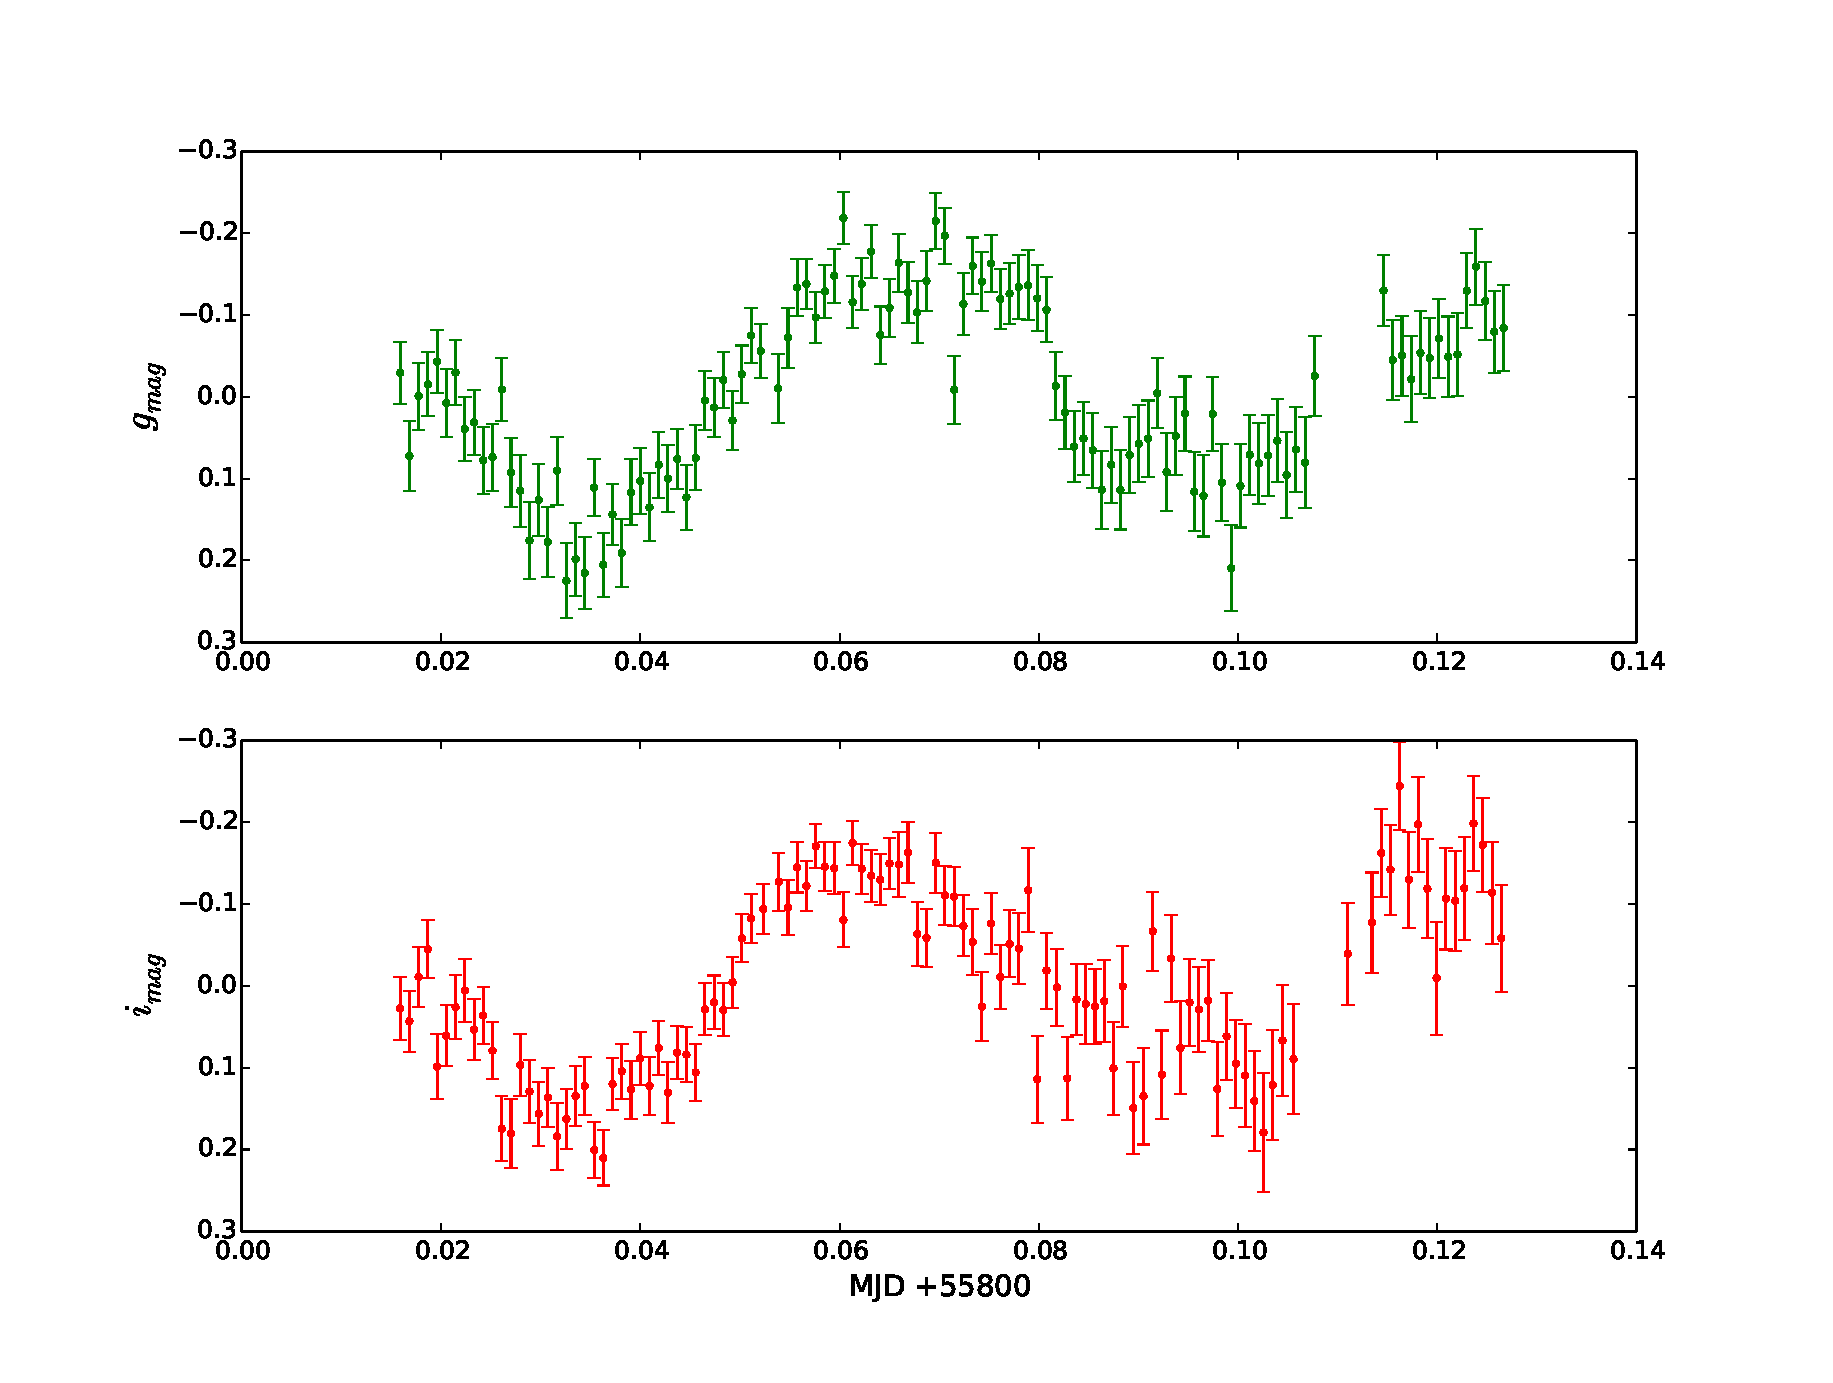
\includegraphics[width=140mm]{images/2011-08-26-run014-110-lightcurve-bin4.eps} 
  \caption{Sloan i, g light curves of asteroid: 2011-08-26-run014-110. Data points are binned by a factor of 4.}
  \label{fig:2011-08-26-run014-110}
\end{figure}


\begin{figure}
  \center
  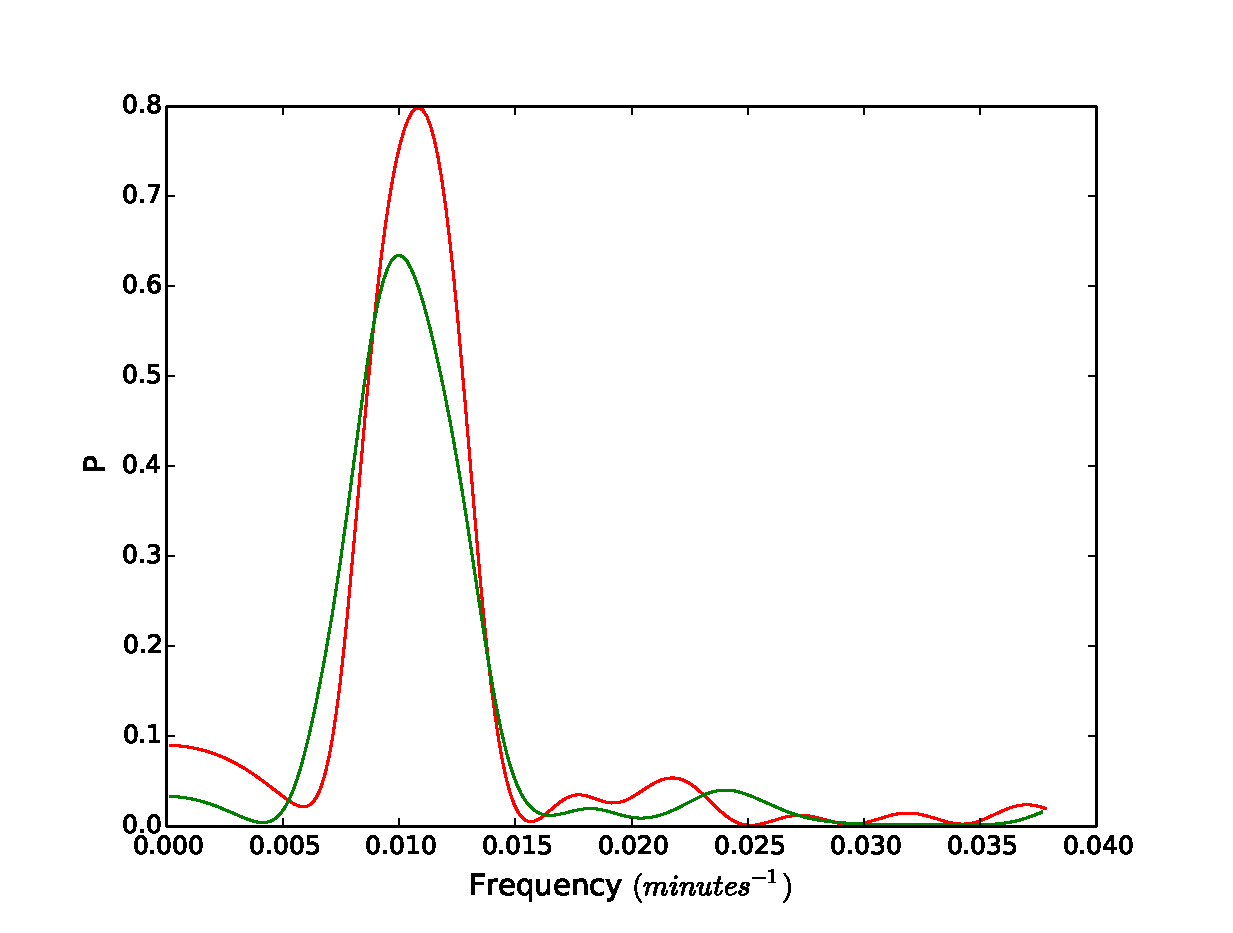
\includegraphics[width=90mm]{images/2011-08-26-run014-110-pgram-bin4.eps} 
  \caption{Periodogram of both the i and g light curves for the object: 2011-08-26-run014-110. The peaks occur at $g_{peak} = 0.0107 \ \mbox{minutes}^{-1}$ and  $r_{peak} = 0.0114\ \mbox{minutes}^{-1}$ }
  \label{fig:asteroidpgram}
\end{figure}

  
%   Classification & Asteroid: 1998 SU139 \\
%   ObjectID & 2011-08-26-run014-110 \\
%   Original target & LY Aqr \\
%   Pixel position & start: (217, 9), end: (505, 54) \\
%   Distance travelled & 291 pixels or 87" \\
%   Field scale & 0.30"/pixel for the WHT\\
%   Duration of run & 12355s (3.43 hours) \\
%   Tangential angular velocity & 0.424"/minute or 25.4"/hour\\ 
%   RA, DEC & MJD=55800.038, 20:51:12, -08:31:25 (J2000) \\
  %URL: & \small \url{http://deneb.astro.warwick.ac.uk/phrnaw/sitedev/2011-08-26/run014.html} \\


The light curve of this object displays a clear sinusoid which must be caused by variations in reflected sunlight that is modulated as the object rotates. A periodogram of these data peaks at a frequency of 0.0114 minutes\textsuperscript{-1} (a spin period of $1.46$ hours) for the 'i' filter and 0.0107 minutes\textsuperscript{-1} (a spin period of $1.56$ hours) for the 'g' filter. This assumes that one period in the light curve is equal to exactly one rotation of the asteroid. This might not be true if the asteroid has several light and dark patches on its surface. 

Rotation of asteroids is driven by a process known as the YORP effect, \citep{yorpeffect}. 

A look-up using the \emph{NEOChecker} tool on the website of the IAU's Minor Planet Center \footnote{http://www.minorplanetcenter.net/cgi-bin/checkneo.cgi} returns a result for this candidate as, most probably, asteroid \emph{1998 SU139}. The world coordinates reported by the tool differed from our own determination by about 6.5'. 

There is a clear relationship between the size of the asteroid and the minimum spin period. It has been shown through observations that, for an asteroid with a diameter greater than 250 metres, the spin period cannot be less than 2.33 hours, \citep{Jacobson2014}. The theoretical reasoning for this 'spin cut-off'  is that, assuming these asteroids are 'rubble-piles' then, above certain angular velocity, the centrifugal forces pulling the rubble pile apart will be stronger than the gravitational forces holding it together and the rubble pile will break up. At the moment, only two asteroids have been found that are exceptions to this rule, \emph{2001 OE84} and \emph{2005 UW163} with periods of 0.486 and 1.290 hours respectively, \citep{Chang2014}. 

  \begin{figure}
    \center
    \includegraphics[width=90mm]{images/jacobson-asteroid-rotation-dot.png} 
    \caption{The spin period distribution as a function of radius for near-Earth (NEA), Mars crossing (MCA) and Main Belt (MBA) asteroids as reported in the Asteroid Lightcurve Database (\cite{2009Icar..202..134W}). The dashed lines indicate the critical surface disruption period $P_d \sim 2.33$ hours for radii $R > 250$ metres. Taken from \cite{Jacobson2014}. The red square on the plot shows the position of our object as estimated in this text.}
    \label{fig:spinrotationcutoff}
  \end{figure}
  

There are several more unconfirmed super-fast rotators (SFR) asteroids reported by \citet{Masiero2009} and \citet{Dermawan2011}. Since these objects have low brightness and fast rotation, periods have not yet been accurately determined. Many of the light curves only have few tens of data points. The fact that we have managed to determine a spin period for this object demonstrates that ULTRACAM is a suitable instrument to use for follow up observations of these other candidates.  

The diameter of the asteroid can be estimated by using its absolute magnitude $H$ and an assumption for the albedo $p$ using the formula, adapted from \citet{Jewitt2013}

$D = \frac{1130}{\sqrt{p}}10^{-H/5} $

We have taken $H = 15.2$ from the JPL Small-Body Database \footnote{http://ssd.jpl.nasa.gov/sbdb.cgi} and assumed an albedo of $ p = 0.297$ for a V-type asteroid. This gives a diameter, $D = 1.89$ km for this asteroid. 

If our period is correct, this could mean that we have discovered a new member of this rare, fast rotator class of asteroid. 

\subsection{Asteroid: 910 Toruyusa}
  
This asteroid was discovered moving through the field of an ULTRACAM run from 
% Classification & Asteroid: 9108 Toruyusa (1997 AZ6) [offset of 7 arc minutes from the computed ephemeris]\\
%   ObjectID & 2009-01-04-run024-61 \\
%   Original target & SDSS J0804+1616 \\
%   Pixel position & start: (137, 422), end: (226, 447) \\
% %   Distance travelled & 92 pixels or 27.6" \\
%   Field scale & 0.30"/pixel for the WHT \\
%   Duration of run & 3221s (53.7 minutes) \\
%   Tangential angular velocity & 0.514"/minute or 31"/hour\\ 
%   RA, DEC & MJD=54836.26642, 08:04:52.3 +16:18:10.6 (J2000) \\
  %URL: & \small \url{http://deneb.astro.warwick.ac.uk/phrnaw/sitedev/2009-01-04/run024.html} \\

  Using the NEOChecker \footnote{http://www.minorplanetcenter.net/cgi-bin/checkneo.cgi} tool, the object detected in this run appears to be a well known asteroid, 9108 Toruyusa. The light curve, which lasts approximately 1 hour shows no significant variation and it has not been possible to determine a spin period for this asteroid.  

  
